\documentclass[MTech,thesis]{iitmdiss}
\usepackage{etex}
%%%%%%%%%%%%%%%%%%%%%%%%%%%%%%%%%%%%%%%%%%%%%%%%%%%%%%%%%%%%%%%%%%%%%%%%%%%%%%%%%%%%%%%%%%%%%%%%%%%%%%%%%

\usepackage[dvips]{graphicx}
\usepackage{amsmath,amssymb} % easier math formulae, align, subequation
\usepackage{fullpage}
\usepackage{graphicx}
\usepackage{amsmath,amssymb,bm}
\usepackage{times,algorithm,algcompatible}
\usepackage{t1enc}
\usepackage{epstopdf}
\usepackage{hyperref}
\usepackage{pstricks,pst-node,pst-tree,pstricks-add}
\usepackage{tikz}
\usepackage{color}
\usepackage{setspace}
\usepackage{bold-extra}
\usepackage{multicol}
\usepackage{caption}
\usepackage{subcaption}
\usepackage{listings}
\usepackage{verbatim}
\usepackage{clrscode3e}
% \usepackage[english,greek]{babel}
\usepackage{ucs} 
% \usepackage[utf8x]{inputenc}
% \usepackage[usenames,dvipsnames]{xcolor}
\usepackage{tikz}
\usepackage{tkz-tab}
\usepackage{caption}
\usepackage{latexsym}
\usepackage{amssymb}
\usepackage{amsmath}
\usepackage{subcaption}
\usetikzlibrary{intersections,decorations, positioning,
arrows,backgrounds,patterns,matrix,shapes,fit,calc,shadows,plotmarks}
%%%%%%%%%%%%%%%%%%%%%%%%%%%%%%%%%%%%%%%%%%%%%%%%%%%%%%%%%%%%%%%%%%%%%%%%%%%%%%%%%%%%%%%%%%%%%%%%%%%%%%%%%%

\newtheorem{theorem}{Theorem}
\newtheorem{corollary}[theorem]{Corollary}
\newtheorem{lemma}[theorem]{Lemma}
\newtheorem{observation}[theorem]{Observation}
\newtheorem{proposition}[theorem]{Proposition}
\newtheorem{definition}[theorem]{Definition}
\newtheorem{claim}[theorem]{Claim}
\newtheorem{fact}[theorem]{Fact}
\newtheorem{assumption}[theorem]{Assumption}
                   %%%%%%%%%%%%%%%%%%%%%%%%%%%%%%%%%%%%%%%%%%%%%%%%%%%%%%%%%
\newcommand{\qed}{\rule{7pt}{7pt}}
\newenvironment{proof}{\noindent{\bf Proof}\hspace*{1em}}{\hfill\qed\bigskip}

\captionsetup{labelfont=bf}

\lstset{
  %backgroundcolor = \color{lightgray},
  frame=single,
  numbers=left,
  numbersep=5pt,
  xleftmargin=2em,
  framexleftmargin=1.5em,
  stepnumber=1,
  firstnumber=1,
  numberfirstline=true,
  basicstyle=\fontsize{10.2pt}{12pt}\ttfamily
}

\hypersetup{
    colorlinks=true, %set true if you want colored links
    linktoc=all,     %set to all if you want both sections and subsections linked
    linkcolor=black,  %choose some color if you want links to stand out
    citecolor=black,
}

%%%%%%%%%%%%%%%%%%%%%%%%%%%%%%%%%%%%%%%%%%%%%%%%%%%%%%%%%%%%%%%%%%%%%%%%%%%%%%%%%%%%%%%%%%%%%%%%%%%%%%%%%%%%%%
%%			AUTHOR DEFINED COMMANDS AND MACROS
%%%%%%%%%%%%%%%%%%%%%%%%%%%%%%%%%%%%%%%%%%%%%%%%%%%%%%%%%%%%%%%%%%%%%%%%%%%%%%%%%%%%%%%%%%%%%%%%%%%%%%%%%%%%%%
\newlength{\LPlhbox}
\newcommand\problemfont[1]{{\scshape #1}}
\newcommand\problemfontbold[1]{\large {\textbf{\textsc{#1}}}}
\renewcommand*\lstlistingname{Algorithm}


\newcommand\segment[4]{
\coordinate (#3) at (#1);
\coordinate (#4) at (#2);
\path (#3) edge[|-|] (#4);
}

\newcommand\lblsegment[5]{
\coordinate (#3) at (#1);
\coordinate (#4) at (#2);
\path (#3) edge[|-|] node[above] {#5} (#4) ;
}

\newcommand\lblsegmenttwo[5]{
\coordinate (#3) at (#1);
\coordinate (#4) at (#2);
\path (#3) edge[|-|] node[at start, above] {#5} (#4) ;
}

\newcommand\lblsegmentthree[5]{
\coordinate (#3) at (#1);
\coordinate (#4) at (#2);
\path (#3) edge[|-|] node[left] {#5} (#4) ;
}

\newcommand\lblsegmentfour[5]{
\coordinate (#3) at (#1);
\coordinate (#4) at (#2);
\path (#3) edge[|-|] node[right] {#5} (#4) ;
}

\newcommand\dashsegment[4]{
\coordinate (#3) at (#1);
\coordinate (#4) at (#2);
\path (#3) edge[|-|,dashed] (#4);
}

\newcommand\lblsegmentdir[6]{
\coordinate (#3) at (#1);
\coordinate (#4) at (#2);
\path (#3) edge[|-|] node[#6] {#5} (#4) ;
}

\newcommand\segmenttwo[4]{
\coordinate (#3) at (#1);
\coordinate (#4) at (#2);
\path (#3) edge[-] (#4);
}

\newcommand\invsegment[4]{
\coordinate (#3) at (#1);
\coordinate (#4) at (#2);
\path [opacity = 0] (#3) edge (#4);
}

\newsavebox{\tempbox}
\newcommand{\cbox}[2]{%
  \fcolorbox{black}{#1}{\texttt{#2\strut}}\kern-\fboxrule}% Coloured box
  
%%%%%%%%%%%%%%%%%%%%%%%%%%%%%%%%%%%%%%%%%%%%%%%%%%%%%%%%%%%%%%%%%%%%%%%%%%%%%%%%%%%%%%%%%%%%%%%%%%%%%%%%%%%%%%


%%%%%%%%%%%%%%%%%%%%%%%%%%%%%%%%%%%%%%%%%%%%%%%%%%%%%%%%%%%%%%%%%%%%%%%%%%%%%%%%%%%%%%%%%%%%%%%%%%%%%%%%%%%%%%
%\setcounter{tocdepth}{4}
%%%%%%%%%%%%%%%%%%%%%%%%%%%%%%%%%%%%%%%%%%%%%%%%%%%%%%%%%%%%%%%%%%%%%%%%%%%%%%%%%%%%%%%%%%%%%%%%%%%%%%%%%%%%%%%

\def\thesistitle{An Improved Implementation of the Approximation Algorithm for the Steiner Tree Problem}
\def\thesisauthor{Anil Kumar}

\begin{document}
%\bibliographystyle{plain}
%%%%%%%%%%%%%%%%%%%%%%%%%%%%%%%%%%%%%%%%%%%%%%%%%%%%%%%%%%%%%%%%%%%%%%
% Title page

\title{\thesistitle}
\author{\thesisauthor}
\date{MAY 2015}
\department{COMPUTER SCIENCE AND ENGINEERING}
%\nocite{*}
\maketitle

%%%%%%%%%%%%%%%%%%%%%%%%%%%%%%%%%%%%%%%%%%%%%%%%%%%%%%%%%%%%%%%%%%%%%%
% Certificate
\certificate

\vspace*{0.5in}

\noindent This is to certify that the thesis titled {\bf {\thesistitle}}, submitted by {\bf {\thesisauthor}}, to the Indian Institute of Technology,
Madras, for the award of the degree of {\bf Master of Technology }, is a bonafide record of the research work done by him under my
supervision. The contents of this thesis, in full or in parts, have not been submitted to any other Institute or University for the award of any
degree or diploma.

\vspace*{1in}
\hspace*{-0.25in}
\begin{singlespace}
\noindent {\bf Dr. N. S. Narayanswamy}\\
\noindent Research Guide\\ 
\noindent Associate Professor\\
\noindent Dept. of Computer Science and Engineering\\
\noindent IIT-Madras, 600 036 \\
\end{singlespace}
\vspace*{0.20in}
\noindent Place: Chennai\\ 
Date: May, 2015


%%%%%%%%%%%%%%%%%%%%%%%%%%%%%%%%%%%%%%%%%%%%%%%%%%%%%%%%%%%%%%%%%%%%%%
% Acknowledgements
\acknowledgements
The work done in this thesis under the guidance of Dr. N. S. Narayanaswamy. I would like to thank Dr. N. S. Narayanaswamy for his guidance and content motivation. He supported me in different roles. I like his friendly behaviour. He given continuous feedback to improve my writing as well as presentation skills. I would once again like to express my deepest gratitude to Dr. N.S. Narayanaswamy for being my mentor.

I would like to my gratitude to some of my friends, they helped me a lot and encouraged me through out my project work. they have given their full support for resolving several of my technical and non-technical doubts. 

I thank all the professors of Computer Science Department, IIT Madras for providing the excellent teaching in the courses. It has helped a lot to understand the key ideas of various fields and their applications. I also appreciate the dedication of staff members of the Department of Computer Science, IIT Madras, for providing every possible facility to the students.
Furthermore I want to thank all my friends I found in IIT Madras, who spent plenty of time with me inside and outside the campus and made me enjoy my time in IIT.
 


\hfill Anil Kumar
%%%%%%%%%%%%%%%%%%%%%%%%%%%%%%%%%%%%%%%%%%%%%%%%%%%%%%%%%%%%%%%%%%%%%%
% Abstract
\abstract

\noindent KEYWORDS: \hspace*{0.5em} \parbox[t]{4.4in}{Graphs, Minimum Spanning Tree, Terminal Steiner Tree, All-pairs Shortest-Path, 
\mbox{Steiner Tree Problem}}

\vspace*{24pt}
\noindent
 \emph{Steiner Tree Problem} ($\textsc{STP}$) Steiner tree problem (named after Jacob Steiner) one of the NP-Complete Problems. If we apply restriction on the problem than we can solved some of the problems in polynomial time. This problem is some what similar to the minimum spanning tree problem. In mst problem, we are required construct a tree that cover all the vertices of a graph with minimum cost. while in the Steiner tree problem, we are given some vertices, which we called as the terminals(required vertices) and some other points which are the optional points(Steiner Point), we are required to connect all the terminal vertices with minimum cost and in this connection, we may use some optional points(Steiner Point) to cover all the terminal vertices with minimum cost.

Given a graph G = $(V,E)$ with edge weights as c:E$\rightarrow$ $\mathbb{R}_{\geq 0}$ i.e, and subset of nodes $S$ $\subseteq$ $V$, $S$ is call required vertices (terminals), formed a tree $T_s$ that cover every required vertices(S) with optimal cost $c(T_s):= \sum_{e\in T_s} c(e)$. This constructed tree $T_s$, we called as the Steiner tree, it might contain some other vertices which are optional(Steiner nodes). Terminal Steiner tree is a tree that having all required vertices as leaves i.e, all the vertices which having degree one are the required vertices. The cost of tree is define as the sum of all the edges cover the path in the construction of tree, this cost is minimum than the other tree, we called such a tree as the minimum cost and there is no other tree, which have cost less then that tree.Even for unit weighted graph this problem is NP-Hard.

\pagebreak


%%%%%%%%%%%%%%%%%%%%%%%%%%%%%%%%%%%%%%%%%%%%%%%%%%%%%%%%%%%%%%%%%
% Table of contents etc.

\begin{singlespace}
\tableofcontents
\thispagestyle{empty}

\listoftables
%\addcontentsline{toc}{chapter}{LIST OF TABLES}
\listoffigures
\addcontentsline{toc}{chapter}{LIST OF FIGURES}
\end{singlespace}


%%%%%%%%%%%%%%%%%%%%%%%%%%%%%%%%%%%%%%%%%%%%%%%%%%%%%%%%%%%%%%%%%%%%%%
% Abbreviations
\abbreviations
 
\noindent 
\begin{tabbing}
xxxxxxxxxxx \= xxxxxxxxxxxxxxxxxxxxxxxxxxxxxxxxxxxxxxxxxxxxxxxx \kill
\textbf{STP}   \> Steiner Tree Problem \\
\textbf{BCR}   \> Bidirected Cut Relaxation \\
\textbf{APSP}   \> All-pairs Shortest-Path\\
\textbf{DFS}   \> Depth First Search\\


\end{tabbing}

\pagebreak


%%%%%%%%%%%%%%%%%%%%%%%%%%%%%%%%%%%%%%%%%%%%%%%%%%%%%%%%%%%%%%%%%%%%%%
% Notation
\chapter*{\centerline{NOTATIONS}}
\addcontentsline{toc}{chapter}{NOTATIONS}
\begin{singlespace}
\begin{tabbing}
xxxxxxxxxxxxxxxxxxxxx \= xxxxxxxxxxxxxxxxxxxxxxxxxxxxxxxxxxxxxxxxxxxxxxxx \kill
\textbf{$G$}		\> Graph \\
\textbf{$T_s$}		\> Minimum Steiner Tree  \\
\textbf{$c(T_s)$}   \> Minimum cost of tree   \\
\textbf{$S$}		\> Require vertices in $G$  \\
\textbf{$A\in B$}	\> All elements of $A$ are present in $B$ \\
% \textbf{$adj(v)$}	\> Set of adjacent vertices of vertex $v$ in the given graph $G$ \\
% \textbf{$deg_G(v)$}	\> Cardinality of $adj(v)$ \\
\textbf{$dist(u,v)$}	\> Distance between $u$ and $v$ in $G$ \\
\textbf{$MST$}	\> Minimum Spanning Tree \\

\end{tabbing}
\end{singlespace}
\pagebreak
\clearpage


\pagenumbering{arabic}
\chapter{INTRODUCTION}
%Chapter 1
%%%%%%%%%%%%%%%%%%%%%%%%%%%%%%%%%%%%%%%%%%%%%%%%%%%%%%%%%%%%%%%%%%%%%%%%%%%%%%%%%%%%%%%%%%%%%%%%%%%%%%%%%%%%%%%%%%%%%%
 In This thesis, we are presenting the study on two problems, $Steiner Tree$ and $All$-$pair$ $shortest$-$path$ problem, and with the help of 
 all-pairs shortest-path, we will reduce the running time of approximation algorithms for Steiner tree. Mainly we will focus on Steiner Tree problems. In this chapter, we present a brief introduction to both the problems. Also, some preliminaries and basic definitions that are used throughout this thesis. And what are the present approximation algorithms for the Steiner tree, which are fastest algorithms for constructing a minimum Steiner tree for a given graph $G$.
 
 \section{Overview and Motivation}
 \subsection{Steiner Tree Problem}
 $\emph{Steiner Tree Problem}$ $(\textsc{STP})$  Problem of Steiner tree is one of the combinatorial optimization problem, which is used in a number of applications, applications in an area like in which some items or points having some common property, we called these types of items or points as the required points in perspective of Steiner tree. So we are required to find the interconnections between these require points with minimum weight or cost of covering these points. While eliminating some unnecessary points, we can use these points, in the formation if these points, helping in construction of the minimum Steiner tree.

 $\textsc{STP}$ problem can be defined as follows:
 
 \begin{tabular}{|ll|}
 \hline
 \multicolumn{ 2}{|l|}{\problemfontbold{Steiner Tree Problem($\textsc{STP}$)}} \\
 \emph{INPUT} & \begin{minipage}[t]{0.75\columnwidth}
 Given a connected undirected graph $G$ = $(V,E)$ and weight of edges\\ $c$:$E$ $\rightarrow$ $\mathbb{R}_{\geq 0}$, a subset of nodes $S$ $\subseteq$ $V$, where $S$ is called as the required\\ vertices(Terminals) given as the input.
 \end{minipage} \\
 \emph{OUTPUT} & \begin{minipage}[t]{0.75\columnwidth}
 A Steiner Tree $T_s$, for Graph $G$ and $S$.
 \end{minipage}
 \\
 \hline
 \end{tabular}
 \\

 Finding the shortest path between two places is an important problem in real life applications and technology. The shortest path problem is also studying in the context of the communication networks. In communication networks, it is important to send data from one hub to other through a shortest available path. In the twentieth century, the development of communication networks forced researchers to design more efficient algorithms for better communication. Here we are presenting some motivational application of Steiner tree problem. Suppose, India want to start some new communication technology between some cities, Let technology is very useful for country, but installation may be costly, but have to start this technology, suppose Indian government is thinking of starting this technology in four major city like Delhi, Mumbai, Kolkata and Chennai, but starting this communication direct to direct from one city to other city it may be costly in some situation like direct linking between cities, there may be a chance of reducing the cost of communication and installation by using some other cities as the intermediary for providing connection between these four cities.

 This type of problem comes under the category of Steiner tree problem, as in Steiner tree problem we are given the required nodes and some non-required nodes, we have to find the connection between the required nodes with minimum cost of interconnection, in this connection we can use some of the non-required nodes. Same case in Steiner tree problem, in that we have to find a minimum cost tree connecting between all the required vertices, these required vertices called terminal vertices, these nodes are basically a subset of the nodes of the connected undirected, weighted graph $G$. Steiner tree problem is NP-Hard. Unless P=NP, there is no polynomial time algorithm for finding optimal solution for Steiner tree problems, so we cannot use well known currently available algorithms for finding an optimal solution of the problems. If we applied some constraints on these problems, then we may be a chance of solving some of the problems in polynomial time. So we have to think for solution in different way, our focus is to find a better algorithm for solving the problems, but there is no polynomial time algorithm for solving NP-Hard problems in polynomial time, so we have to change our approach for solving these problems, so now we are focusing on the better approximation algorithms with good running time.

  Till now best known approximation bound for Steiner tree problems is 1.55 given by Robins and Zelikovsky[2000]~\cite{hougardy}. There is no improvement for a long time in this Approximation, So we have to think problem differently to get the best approximation. For this our focus is on the LP-Based approximation like directing-component cut relaxation and Iterative randomized rounding. By LP-Based we are getting an approximation (ln 4 + $\in$) factor for some graph~\cite{byrka}.

  In this report our focus is to get the better run time for approximation algorithms. We will test the algorithm by running a test instance provided for the Steiner tree.\\


 \begin{tabular}{|ll|} 
 \hline
 \multicolumn{ 2}{|l|}{\problemfontbold{Steiner Tree Problems}} \\
 \emph{GOAL} & \begin{minipage}[t]{0.75\columnwidth}
 A MST that cover all the required vertices with minimum cost.
 \end{minipage} \\
 \emph{INPUT} & \begin{minipage}[t]{0.8\columnwidth}
 A connected undirected graph $G$ = $(V,E)$ with edge costs $c$:$E$ $\rightarrow$ $\mathbb{R}_{\geq 0}$,\\ and a subset of nodes $S$ $\subseteq$ $V$,  $S$ is called as the required nodes.
 \end{minipage} \\
 \emph{OUTPUT} & \begin{minipage}[t]{0.75\columnwidth}
 A Steiner Tree $T_s$, for Graph $G$ and $S$.
 \end{minipage}
 \\
 \hline
 \end{tabular}
 \\

 In figure 1.1, dark vertices are representing the required vertices, while hollow vertices representing the Steiner vertices, so we are required to cover every required vertices of the graph $G$ with the optimal cost, cost is the total sum of the edge weight that are participating in the Steiner tree formation. In figure 1.2, dark edges represent the Steiner tree that cover every terminal(require) vertices by using some of the Steiner vertices, the cost of covering all the require vertices is minimum, as there is no other tree that cover all the require vertices minimum cost which is less than that, and cover all the require vertices.

% \begin{figure}
%\begin{center}
\begin{figure}
\begin{center}
\centering
\begin{tikzpicture}[shorten >=1pt, auto, node distance=2cm,
   node_style/.style={circle,draw=black,minimum size = 20pt},
   edge_style/.style={draw=black, ultra thick}]

    \node[node_style] (v1) at (-1,0) {h};
    \node[node_style, fill=black!40] (v2) at (-4, 0) {a};
    \node[node_style] (v3) at (2,0)  {k};
    \node[node_style,fill=black!40] (v4) at (5,0)  {d};

    \node[node_style] (v5) at (-3,2) {g};
    \node[node_style] (v6) at (0,2)  {f};
    \node[node_style] (v7) at (-3,-3) {j};
    \node[node_style] (v8) at (-2,-1) {i};
    \node[node_style,fill=black!40] (v9) at (0,-3)  {b};
    \node[node_style] (v10) at (2,-2) {l};
    \node[node_style,fill=black!40] (v11) at (4,-3) {c};
    \node[node_style,fill=black!40] (v12) at (3,2)  {e};
    \draw[edge_style]  (v2) edge node{10} (v5);
    \draw[edge_style]  (v2) edge node{1} (v1);
    \draw[edge_style]  (v2) edge node{4} (v7);
    \draw[edge_style]  (v1) edge node{2} (v3);
    \draw[edge_style]  (v1) edge node{2} (v8);
    \draw[edge_style]  (v1) edge node{1} (v5);
    \draw[edge_style]  (v8) edge node{1} (v7);
    \draw[edge_style]  (v7) edge node{1} (v9);
    \draw[edge_style]  (v9) edge node{2} (v3);
    \draw[edge_style]  (v9) edge node{1} (v10);
    \draw[edge_style]  (v3) edge node{2} (v4);
    \draw[edge_style]  (v3) edge node{1} (v10);
    \draw[edge_style]  (v11) edge node{1} (v10);
    \draw[edge_style]  (v4) edge node{10} (v12);
    \draw[edge_style]  (v4) edge node{9} (v11);
    \draw[edge_style]  (v3) edge node{1} (v6);
    \draw[edge_style]  (v5) edge node{2} (v6);
    \draw[edge_style]  (v12) edge node{1} (v6);
    \draw[edge_style]  (v9) edge node{8} (v11);
    \end{tikzpicture}
    \caption{\small \sl A connected Graph $G$, with edges weights, having Steiner vertices(hallow) and terminal vertices(dark) \label{fig:sccEx} }
    \end{center}
    \end{figure}
\begin{figure}
\begin{center}
\begin{tikzpicture}[shorten >=1pt, auto, node distance=2cm, 
   node_style/.style={circle,draw=black,minimum size = 20pt},
   edge_style/.style={draw=black, ultra thick}]

    \node[node_style] (v1) at (-1,0) {h};
    \node[node_style, fill=black!40] (v2) at (-4, 0) {a};
    \node[node_style] (v3) at (2,0)  {k};
    \node[node_style,fill=black!40] (v4) at (5,0)  {d};

    \node[node_style] (v5) at (-3,2) {g};
    \node[node_style] (v6) at (0,2)  {f};
    \node[node_style] (v7) at (-3,-3) {j};
    \node[node_style] (v8) at (-2,-1) {i};
    \node[node_style,fill=black!40] (v9) at (0,-3)  {b};
    \node[node_style] (v10) at (2,-2) {l};
    \node[node_style,fill=black!40] (v11) at (4,-3) {c};
    \node[node_style,fill=black!40] (v12) at (3,2)  {e};
    \draw[edge_style]  (v2) edge node{10} (v5);
    \draw[edge_style, line width=4pt]  (v2) edge node{1} (v1);
    \draw[edge_style]  (v2) edge node{4} (v7);
    \draw[edge_style, line width=4pt]  (v1) edge node{2} (v3);
    \draw[edge_style]  (v1) edge node{2} (v8);
    \draw[edge_style]  (v1) edge node{1} (v5);
    \draw[edge_style]  (v8) edge node{1} (v7);
    \draw[edge_style]  (v7) edge node{1} (v9);
    \draw[edge_style]  (v9) edge node{2} (v3);
    \draw[edge_style, line width=4pt]  (v9) edge node{1} (v10);
    \draw[edge_style, line width=4pt]  (v3) edge node{2} (v4);
    \draw[edge_style, line width=4pt]  (v3) edge node{1} (v10);
    \draw[edge_style, line width=4pt]  (v11) edge node{1} (v10);
    \draw[edge_style]  (v4) edge node{10} (v12);
    \draw[edge_style]  (v4) edge node{9} (v11);
    \draw[edge_style, line width=4pt]  (v3) edge node{1} (v6);
    \draw[edge_style]  (v5) edge node{2} (v6);
    \draw[edge_style, line width=4pt]  (v12) edge node{1} (v6);
    \draw[edge_style]  (v9) edge node{8} (v11);
    \end{tikzpicture}
    % \caption{\small \sl Torricelli point X \label{fig:sccEx} }
    \end{center}
    \caption{\small \sl A Graph G, with edges weights and Steiner vertices as hollow vertices, terminal vertices(dark) and Steiner tree(dark edges) \label{fig:sccEx} }
    \end{figure}
\subsection{Terminal Steiner Tree}
 For a given graph $G$, Steiner tree whose all terminal vertices are of degree one, i.e., all the required vertices which are covered by the tree to form Steiner tree of minimum cost are leaves. All the require nodes of the Steiner tree must be leaves, but there is no restriction on the require nodes in the Steiner tree. In Steiner tree terminal node can also be some internal node. For example, in figure 1.3(a), a Steiner tree is formed from the a given graph $G$, in that Steiner tree some of the internal nodes are also terminal node. While in figure 1.3(b), a Steiner tree all the required vertices are leaves only, so this Steiner tree is called as the terminal Steiner tree.\\

 \begin{tabular}{|ll|} 
 \hline
 \multicolumn{ 2}{|l|}{\problemfontbold{Terminal Steiner Tree}} \\
 \emph{INPUT} & \begin{minipage}[t]{0.8\columnwidth}
  A connected weighted graph $G$ = $(V,E)$ with edge costs $c$:$E$ $\rightarrow$ $\mathbb{R}_{\geq 0}$, and\\ a subset of nodes $S$ $\subseteq$ $V$, $S$ is call required vertices (Terminals) as a input.
 \end{minipage} \\
 \emph{Output} & \begin{minipage}[t]{0.8\columnwidth}
 A Steiner tree $T_s$ of $G$, such that all the terminal node must be of degree one.
 \\	
 \end{minipage}
 \\
 \hline
 \end{tabular}
 
 \begin{figure}
\centering
\begin{subfigure}{.5\textwidth}
  \centering
    \begin{tikzpicture}[shorten >=1pt, auto, node distance=2cm,
            node_style/.style={circle,draw=black,minimum size = 10pt},
            edge_style/.style={draw=black, ultra thick}]
    \node[node_style] (v1) at (0,0.5)  {a};
    \node[node_style,fill=black!50] (v2) at (-2,-1) {b};
    \node[node_style] (v3) at (2,-1)  {c};
    \node[node_style,fill=black!50] (v4) at (2,2) {d};
    \node[node_style,fill=black!50] (v5) at (-2,2) {e};
    \node[node_style,fill=black!50] (v6) at (4,0.5) {f};

    \draw[edge_style, line width=4pt]  (v1) edge node{2} (v2);
    \draw[edge_style]  (v1) edge node{2} (v3);
    \draw[edge_style, line width=4pt]  (v1) edge node{2} (v4);
    \draw[edge_style, line width=4pt]  (v1) edge node{2} (v5);
    \draw[edge_style]  (v2) edge node{10} (v5);
    \draw[edge_style]  (v2) edge node{10} (v3);
    \draw[edge_style]  (v5) edge node{10} (v4);
    \draw[edge_style]  (v4) edge node{10} (v3);
    \draw[edge_style, line width=4pt]  (v4) edge node{2} (v6);
    \draw[edge_style]  (v3) edge node{2} (v6);
    \end{tikzpicture}
  
  % \includegraphics[width=.4\linewidth]{image1}
  \caption{Steiner tree of a graph with four terminals}
  \label{fig:sub1}
\end{subfigure}%
\begin{subfigure}{.5\textwidth}
  \centering
  \begin{tikzpicture}[shorten >=1pt, auto, node distance=2cm,
            node_style/.style={circle,draw=black,minimum size = 10pt},
            edge_style/.style={draw=black, ultra thick}]
    \node[node_style] (v1) at (0,0.5)  {a};
    \node[node_style,fill=black!50] (v2) at (-2,-1) {b};
    \node[node_style] (v3) at (2,-1)  {c};
    \node[node_style,fill=black!50] (v4) at (2,2) {d};
    \node[node_style,fill=black!50] (v5) at (-2,2) {e};
    \node[node_style,fill=black!50] (v6) at (4,0.5) {f};

    \draw[edge_style, line width=4pt]  (v1) edge node{2} (v2);
    \draw[edge_style, line width=4pt]  (v1) edge node{2} (v3);
    \draw[edge_style, line width=4pt]  (v1) edge node{2} (v4);
    \draw[edge_style, line width=4pt]  (v1) edge node{2} (v5);
    \draw[edge_style]  (v2) edge node{10} (v5);
    \draw[edge_style]  (v2) edge node{10} (v3);
    \draw[edge_style]  (v5) edge node{10} (v4);
    \draw[edge_style]  (v4) edge node{10} (v3);
    \draw[edge_style]  (v4) edge node{2} (v6);
    \draw[edge_style, line width=4pt]  (v3) edge node{2} (v6);
    \end{tikzpicture}
  
  % \includegraphics[width=.4\linewidth]{image1}
  \caption{Terminal Steiner tree of a Graph G}
  \label{fig:sub2}
\end{subfigure}
\caption{Terminal Steiner Tree in which all the degree vertices are terminals, while in case of Steiner tree some internal node can also be terminal nodes.}
\label{fig:test}
\end{figure}
\section{Applications of Steiner Tree}
 The Steiner tree problems have so many applications like in circuit layout, network design, and telephone communications. Everywhere where the shortest path required between the interconnecting, some of the require points with some specific properties and we are required to connect these points with the help of some optional points, there we can use Steiner tree.
  Here are the some applications of Steiner tree.\\
 \textbf{In physical VLSI designs:-}
  Steiner tree is used, whenever the placement of component on a chip, there may be a chance that, a set of pin are to be connected with in the free space. A set pin which sharing the networks in the designs, these pins are called as the required vertices, and some other pins which are not useful in the network designs, but with the help of these pins we may connect the require vertices in designing of the network. with the help of these optional pins, we may connect the required pins and fulfil the purpose of the require pins in the designs of networks.\\
 \textbf{On-line and Dynamic Steiner tree:-}
 On-line application of the Steiner tree comes, whenever a new change in the network because of some new additional points for service, then there is a requirement of new connection in the telephone network. If a new points for the service is added then, a new line of connect for the new point in the network has to build. In this network construction is like a way the every time, whenever location is change a new network is formed based on the previous network. this brings us a issue of dynamic Steiner tree, in that whenever new network is built, we have to calculate an approximation for the performance of the network.
 \section{Existing Approximation Algorithms}
 There are series of research in the improvement the approximation ratio of the Steiner tree problems. It starts from 2-approximation and after so many of the  improvement it reached to 1.55, i.e., the best known approximation by Robins and Zelikovsky[2000] ~\cite{hougardy}.\\\
Here is the list of Existing approximation ratio for the Steiner tree ~\cite{hougardy}.\\
\begin{table}[h]
% \caption{My caption}
\label{my-label}
\begin{center}
\begin{tabular}{|l|l|l|l|l|l|l|l|l|}
\hline
Approximation Bound & References \\ \hline
    2.0-approximation  & minimum spanning tree heuristic \\ \hline
    1.83-approximation & Zelikovsky 1993   \\ \hline
    1.78-approximation & Berman and Ramaiyer 1994 \\ \hline
    1.73-approximation & Borchers and Du 1997 \\ \hline
    1.67-approximation & Pr\"{o}mel and Steger 1997 \\ \hline
    1.65-approximation & Karpinski and Zelikovsky 1997 \\ \hline
    1.59-approximation & Hougardy and Pro\"{o}mel 1999 \\ \hline
    1.55-approximation & Robins and Zelikovsky 2000 \\ \hline

         % &        &        &        &           &        &        &       &          \\ \hline
         % &        &        &        &           &        &        &       &          \\ \hline
\end{tabular}
\end{center}
\caption{Existing approximation ratio for the Steiner tree}
\end{table}
A series of improvement, maximize with Robins and Zelikovsky's ~\cite{byrka} famous 1+$\frac{ln(3)}{2}$ + $\epsilon$ $<$ 1.55 (here $\epsilon$ $>$0 is an arbitrary small constant) algorithm improved this ratio by iteratively improving upon the minimum weight terminal Steiner tree. The above results are based on the Steiner tree as a full components. A component of the Steiner tree is the tree whose all the required(terminal) vertices are the leaves of the tree. But considering the full component at a time will not give a good approximation ratio. If we consider the Steiner tree with special structure, So called r-restricted Steiner, in this tree every components that have no more than r-terminals. To get a better approximation, It is better to pay attention to r-restricted Steiner tree. By using this approach we may get a better approximation ratio ~\cite{byrka}.\\
{\textbf{Steiner Ratio:-} The Ratio between the total length of the minimum Steiner tree and the total length of a minimum Spanning tree, Steiner ratio represented as $\rho$.
\section{All-Pairs Shortest-Paths Algorithm}

 All-Pair Shortest-path(APSP) problem is one of the fundamental problems in the graph theory. A classical ways for solving 
 $\textsc{APSP}$ in general weighted graphs is given by Floyd and Warshall ~\cite{cormen}. It outputs an $V$ $\times$ $V$ matrix, in that every pairs of vertices at the minimum distance, it takes $\Theta(V^3)$ time. In all-pairs Shortest-paths problem, 
 we are required to find the shortest path between each and every pairs of vertices of the graph $G$ = $(V,E)$. $i.e.,$ we are given a $V_i$ and $V_j$ where $(V_i,V_j)$ $\in$ $V$, this algorithm used to find the shortest paths between vertices $V_i$,$V_j$. All-Pairs Shortest-Paths problem can be solved by using the a single-source shortest-path algorithm by running $|V|$ times to find the shortest path for each and every vertex of the graph as a source. With the help of All-Pairs Shortest-paths
 algorithms, we are coming up a better running time approximation algorithm for Steiner tree, this algorithm will be better only for those graph which have edges of order $O(E)$ $\leq$ $|V|log|V|$. Running time of an algorithm totally depends 
 on algorithmic and data-structure that we are using in the implementation.   

\section{Preliminaries}

\textbf{Weighted Graph:-} A graph has two elements, vertices and edges. The edges connecting the two end points or vertices of the graph, have some cost of connecting two vertices, this is called as the weight for that edge. If weights are associated with every edge, this type of graph called as the weighted graph. Weight sum of all the edges is called as the weight of graph. \\ 
 \textbf{Path in a Graph:-} A path is a sequence of edges which connects the vertices of the graph. The Sum of all associated weights with edges so called as the weight of the path.\\
 \textbf{Subgraph:-} A subgraph $P$ is the subgraph of the graph $G$, whose edges and vertices are the subset of the $G$.\\
 \textbf{Tree:-} A tree is a acyclic graph. A tree is a graph is which every vertex is connected with exactly one path, one degree vertices are called as the leaves of the tree. Tree became disconnected after removal of any edges.\\
 % \textbf{Degree of the vertices:-} Number of edges connected to a vertex is known as the degree of that vertex.\\
 \textbf{Minimum Spanning Tree:-} A spanning tree of a graph is the tree which connects every vertices of the graph, A minimum spanning tree is the tree which have optimal cost of covering every vertices. i.e., there is no other tree having weight less than a minimum spanning tree. The sum of all the weight of all the edges of tree is called as the weight of the minimum spanning tree. Algorithms for finding the minimum spanning tree in a graph are Prim's algorithm, kruskal's algorithm.\\
 \textbf{Dijkstra's Algorithm:-} Dijkstra's algorithm one of the shortest path algorithm, it use single vertex as a source for finding the shortest path. Run time complexity of this algorithm is $O(|E| + |V|log|V|)$, if we use fibonacci heap as in implementation, where $|E|$ is the number of edges.\\
 \textbf{Sparse Graph:-} A graph in which number of edges are much less than the possible number of edges.
 \section{Contribution of the Thesis}
 In this thesis, we restrict our attention on fastest approximation algorithm for Steiner tree. Not only on the theoretical interest about the approximation algorithm of the Steiner tree, But also on the practical impact of the algorithms are present in this thesis.
 All-Pairs Shortest-Paths algorithms have been shown to find some better solution in practice for approximation algorithm, But because of the high run time on a big graph and different type of problems limits their applicability. Underlying graph structure can play an important role in setting up efficient approximation algorithms. All-pairs shortest-paths algorithms, tries to improve an existing solution by modifying the current exiting algorithm, for finding the best path between the pair of terminals. In this All-pairs shortest paths basically focusing on the find the best minimum path between the terminals, by that it for providing some better  solution for our approximation algorithm, if we apply some change in algorithm. By this way we may get better run time for some limited problems, This is also confirming that non-trivial data-structures and algorithmic are also very important for the solution of some real-world problems for optimization. 
 \section{Organization of the Thesis}
 This thesis is organized in 5 chapters. Current chapter is an introduction to the thesis. It contains an introduction           
 and motivation for the Steiner tree problem. We presented some graph theoretic preliminaries which are used throughout this thesis.
 In Chapter \ref{ch_prelim} we study various types of Steiner tree and existing algorithms, and we explained some of the approximation algorithms. Also, we prove the various important properties of Steiner tree. Chapter \ref{ch_review} presents a nice survey of the work done on all-pairs shortest-path algorithms and how, it will use in the Steiner tree algorithm for improving the running time for heuristic algorithm.
In chapter \ref{ch_distOracle} we present an algorithm to construct a shortest distance between all-pairs of terminals using APSP. How we are using this algorithm to solve the approximation algorithm for Steiner tree. Finally, Chapter \ref{ch_concl} concludes the thesis. This chapter also lists some interesting direction for research and open problems for further study, and some case that can be consider for further improvement in the approximation algorithms.
\chapter{ALL ABOUT STEINER TREE} \label{ch_prelim}
% %Chapter 2
% %%%%%%%%%%%%%%%%%%%%%%%%%%%%%%%%%%%%%%%%%%%%%%%%%%%%%%%%%%%%%%%%%%%%%%
In this chapter, we are presenting all about the Steiner tree problems. In this we will present, what are the properties of the Steiner tree and types of the Steiner tree, which are the algorithms for the different type of Steiner tree and their approximation algorithms.
\section{Steiner Tree}
 The Steiner Tree in a given graph $G = (V,E)$ is a tree that cover all the terminal vertices of the graph with minimum cost, terminals are the subset of the vertices which are required in the connection, i.e., have to be cover in the minimum spanning tree.
 In this section we define and give different type of Steiner tree problems.
\section{Types of Steiner Trees problems}
 Based on the applications and uses the Steiner tree are of the different types. For example, if a Steiner tree is applied in the VLSI network, then this type of Steiner tree so called as the terminal Steiner tree. In this section, we will discuss a few types of Steiner tree Problems.

\subsection{Euclidean Steiner Tree}
 The Euclidean Steiner Problem(ESP) was well researched by Zacharis, the origin of ESP is often traced back to Fermat(1601-1665) 
 who proposed the following problem: We are given some terminal points in the 2-dimensional space and some optional points. Here we considering the cost of connecting the points is same as the distance between the points. Find a point in the plane that sum the connection of minimum distance, and point is in such a way that the sum of whose distances from three given points should be minimal.
  This problem will be referred to as the Fermat problem. In figure 2.1 three points are shown in the Euclidean plane, if we connect these point with help of a Steiner point(shown as hollow in figure) then we will get a tree that covers all these points with minimum distance $\sqrt{3}$. 

  A solution for this problem is given by torricelli in 1640, he gave solution by using some geometric triangle for this problem. He propose that, if we draw three circles using circumscribing of equilateral triangles sides for construction of the circle, these circle meat at point that point called as called the Torricelli point. In figure 2.2, in triangle, a Torricelli point is formed after the intersection of three circles. The circle are drowned at the edges of the equilateral triangle every circle pass through the two points of side of the triangle and the intersection point of these three circles is so called Torricelli point. The distance from the Torricelli point and the give point is called Euclidean distance and the sum of all the distance is minimum.

   Here in this figure 2.1, shown that the solution of the 3 points problem with the Torricelli method, if we found a Torricelli point, we can draw edges having an equal distance from this point to the other point. In this figure 2.1, point form a triangle, if we form a minimum weight tree from this triangle the total cost of that minimum spanning tree will be 2 which is not the minimum cost of covering all points in the plane, and if we form a Steiner minimum tree by taking the Steiner point as the center of these point, then we are getting a tree that covers all points with minimum distance this is so called Steiner tree.

    
\begin{figure}
\centering
\begin{subfigure}{.5\textwidth}
  \centering
  \begin{tikzpicture}[shorten >=1pt, auto, node distance=2cm, ultra thick,
            node_style/.style={circle,draw=black,minimum size = 10pt,font=\sffamily\Large\bfseries},
            edge_style/.style={draw=black, ultra thick}]
    % \node[node_style] (v1) at (0,0)  {a};
    \node[node_style,fill=black!500] (v2) at (-2,-1) {};
    \node[node_style,fill=black!500] (v3) at (2,-1)  {};
    \node[node_style,fill=black!500] (v4) at (0,2) {};
    \end{tikzpicture}
  
  % \includegraphics[width=.4\linewidth]{image1}
  \caption{}
  \label{fig:sub1}
\end{subfigure}%
\begin{subfigure}{.5\textwidth}
  \centering
  \begin{tikzpicture}[shorten >=1pt, auto, node distance=2cm, ultra thick,
            node_style/.style={circle,draw=black,minimum size = 10pt,font=\sffamily\Large\bfseries},
            edge_style/.style={draw=black, ultra thick}]
    % \node[node_style] (v1) at (0,0)  {a};
    \node[node_style,fill=black!500] (v2) at (-2,-1) {};
    \node[node_style,fill=black!500] (v3) at (2,-1)  {};
    \node[node_style,fill=black!500] (v4) at (0,2) {};

    \draw[edge_style]  (v2) edge node{1} (v3);
    \draw[edge_style]  (v2) edge node{1} (v4);
    \draw[edge_style]  (v3) edge node{1} (v4);
    \end{tikzpicture}
  
  % \includegraphics[width=.4\linewidth]{image1}
  \caption{}
  \label{fig:sub2}
\end{subfigure}
% \caption{A figure with two subfigures}
% \label{fig:test}
% \end{figure}
\\

% \begin{figure}
\centering
\begin{subfigure}{.5\textwidth}
  \centering
  \begin{tikzpicture}[shorten >=1pt, auto, node distance=2cm, ultra thick,
            node_style/.style={circle,draw=black,minimum size = 10pt,font=\sffamily\Large\bfseries},
            edge_style/.style={draw=black, ultra thick}]
    % \node[node_style] (v1) at (0,0)  {a};
    \node[node_style,fill=black!500] (v2) at (-2,-1) {};
    \node[node_style,fill=black!500] (v3) at (2,-1)  {};
    \node[node_style,fill=black!500] (v4) at (0,2) {};
    \draw[edge_style]  (v2) edge node{1} (v4);
    \draw[edge_style]  (v2) edge node{1} (v3);
    % \draw[edge_style]  (v5) edge node{10} (v4);
    \end{tikzpicture}
  
  % \includegraphics[width=.4\linewidth]{image1}
  \caption{}
  \label{fig:sub1}
\end{subfigure}%
\begin{subfigure}{.5\textwidth}
  \centering
  \begin{tikzpicture}[shorten >=1pt, auto, node distance=2cm, ultra thick,
            node_style/.style={circle,draw=black,minimum size = 10pt,font=\sffamily\Large\bfseries},
            edge_style/.style={draw=black, ultra thick}]
    \node[node_style] (v1) at (0,0)  {};
    \node[node_style,fill=black!100] (v2) at (-2,-1) {};
    \node[node_style,fill=black!500] (v3) at (2,-1)  {};
    \node[node_style,fill=black!500] (v4) at (0,2) {};
    \draw[edge_style]  (v1) edge node{$\frac{1}{\sqrt{3}}$} (v2);
    \draw[edge_style]  (v1) edge node{$\frac{1}{\sqrt{3}}$} (v3);
    \draw[edge_style]  (v1) edge node{$\frac{1}{\sqrt{3}}$} (v4);
    \end{tikzpicture}
  
  % \includegraphics[width=.4\linewidth]{image1}
  \caption{}
  \label{fig:sub2}
\end{subfigure}
\caption{(a) three points are given in the euclidean plane. (b) these point form triangle suppose edges length is 1 for each. (c) minimum spanning tree of cost 2. (d) Steiner tree form using one Steiner point}
\label{fig:test}
\end{figure}

 \begin{figure}
      \centering
    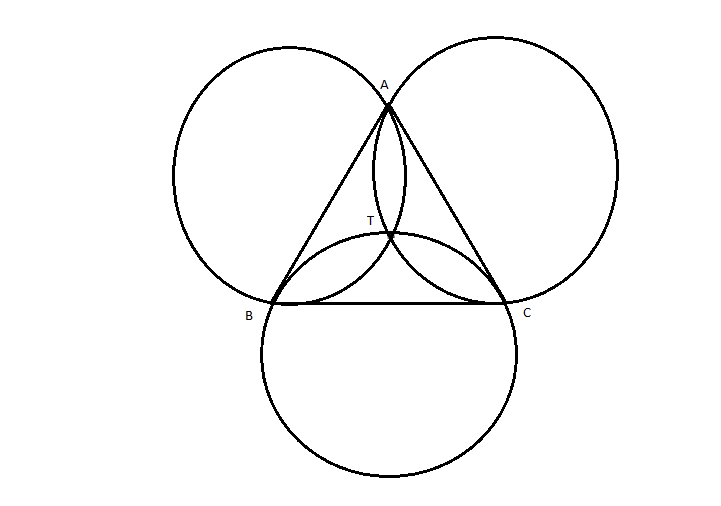
\includegraphics[scale = 0.8]{torr.png}
  \caption{A triangle ABC, and Torricelli Point T (Black dot at the center of the triangle ABC)} intersection of all the circle.
\end{figure}

 Characteristics of this Torricelli point that it always lies inside the triangle and the distance sum from all other point triangle corner to the torricelli point is minimum. If triangle is equilateral triangle than $\angle$ ATC = $\angle$ BTC = $\angle$ CTA = $120$. As Shown in figure 2.2, Circle are draw by taking center as the outside intersection point of arch drown by taking the corner of the triangle edge as a center, by taking that intersection point as center and  draw a circle which passes through the end points of edges, this process is done for all the three circle, the intersection point of these three circle is so called Steiner point or torricelli point.   

 
\subsection{Rectilinear Steiner Problem}
A Steiner tree, whose spanning tree overs a set of points in the collection by using vertical and horizontal lines which covers the points in the given space is called rectilinear tree. These sets of lines are called Steiner trees. The Length of a tree is the weight sum of its lines, and a rectilinear Steiner minimal tree(RSMT) is a tree of minimum length. According the statement by Hanan's we can find the number of Steiner tree exist in a grid, that having the points. This can be drown by horizontal and vertical line than can be form by connecting the set of points that are presents in the plane ~\cite{shen}.

Rectilinear minimum Steiner tree problem is a one of the problem in the geometric plane for the Steiner tree problem, for that we have to replaced euclidean distance by rectilinear distance that form a grid like structure. Given the points there is a interconnections between the points in fashion of horizontal and vertical lines. This arises the application of Steiner tree VLSI design, because in VLSI design there is a linear relationship between the wire-length and wiring area.

In figure 2.3(a), grid structure is given to the four points lies in the rectilinear plane, suppose that the distance from one grid to another grid is 1, from both way horizontal or vertical. In figure 2.3(b), a minimum spanning tree is formed by using these points, the cost of forming minimum spanning tree will be 6, this cost is not minimal cost of covering all the points in rectilinear plane. In figure 2.3(c), we are using one Steiner point(show as hollow) to connect all the required vertices, than the cost of covering all the points will be 4 which is minimum cost of covering all the points. 
 \begin{figure}
      \centering
    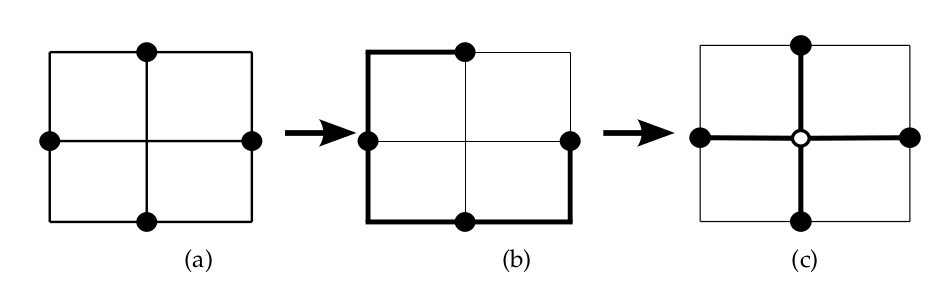
\includegraphics[scale = 0.4]{rec.png}
  \caption{(a) Grid having four terminal point int rectilinear plane (b) minimum spanning tree of cost 6 using all four points (c) minimum Steiner tree of cost 4}
\end{figure}

\subsection{Steiner Tree Problems in Network}
This problem is the combinatorial version of the Euclidean problem for Steiner tree. If $G$ is not connected and terminals appear in 
at least two components, then there is no solution for the Steiner problem. If G is not connected but all terminals appears in one component, then the remaining components can be disregarded and we can get the solution for the by using only the terminals that are present in the component. For this problem in the network by using Steiner tree, it is assumed that the $G$ is connected graph. The Problem of Steiner tree in networks was originally formulated by Hakimiand independently by levinin 1971. After that this problem received considerable attention for the research in the network.\\

 \begin{tabular}{|ll|} 
 \hline
 \multicolumn{ 2}{|l|}{\problemfontbold{Steiner Tree Problem in Network}} \\
 \emph{INPUT} & \begin{minipage}[t]{0.8\columnwidth}
 A undirected graph G = $(V,E)$, edge costs c:E$\rightarrow$ $\mathbb{R}_{\geq 0}$, and a nodes $S \subseteq V$,  $S$ is the subset if vertices, called required nodes.
 \end{minipage} \\
 \emph{OUTPUT} & \begin{minipage}[t]{0.8\columnwidth}
 A Steiner Tree $T_s$, Such that there is a path between every pair of terminals.\\
 \end{minipage}
 \\
 \hline
 \end{tabular}
 \\

\subsection{Prize-Collecting Steiner Tree(PCST)}
The Prize collecting Steiner tree(PCST) in a given undirected graph G, with edges cost and vertex profits. In PCST we form a Steiner tree by using terminal vertices such that it minimizing total sum of the edge's weight in the Steiner tree plus the profit of all the vertices which are not in the Steiner tree.

\begin{tabular}{|ll|} 
 \hline
 \multicolumn{ 2}{|l|}{\problemfontbold{Prize-Collecting Steiner Tree(PCST)}} \\
 \emph{INPUT} & \begin{minipage}[t]{0.8\columnwidth}
 A undirected connected graph $G$ = $(V,E)$ with edge costs $c:E\rightarrow \mathbb{R}_{\geq 0}$, and a $|S|$ nodes $S \subseteq V$,  $|S|$ is so called terminal nodes and $p$ is vertex profit.
 \end{minipage} \\
 \emph{OUTPUT} & \begin{minipage}[t]{0.8\columnwidth}
 A Steiner Tree $T_s$ = $(V_s,E_s)$ of G, $E_s$ $\subseteq$E, that minimize the objective function c(s) =$\sum_{v_{\notin V_s}}p(V)$ + $\sum_{E_{\in E_s}}c(E)$  .\\
 \end{minipage}
 \\
 \hline
 \end{tabular}
 \\


\section{Approximation Algorithm for Steiner Tree}

Here we are presenting the approximation algorithm from a graph $G$ for finding the Steiner tree. A graph $G$ is given with edges weight and a vertex set $|S|$ which, we called as the terminal nodes. Sequence of vertices $(v_1,v_2,v_3 \dots v_k)$ is known as the path in the graph. The Weighted sum of all the edges which are present in the path is known as the weight of the path. A spanning tree is the tree that cover all the vertices of the graph, if the weight of a path is minimum than this tree is so called as the minimum spanning tree. If we applied some conditions on this like, we have to cover some particular nodes, and have to find the minimum distance between these nodes, then these type of cases comes under the category of the Steiner tree problems, in that we have to cover all the terminals, if all the terminals cover by a tree with minimum weight, i.e., there is no other optimal weighted tree which have less weight than of that, this type of tree so called as the minimum Steiner tree.

 Finding a minimum Steiner tree in a graph $G$ and $S$ is the NP-complete problem. So have to think about some approximation solution for these problems. An approximation algorithm best known for Steiner tree problems. We start with a heuristic algorithm that can be use for finding the Steiner tree from a given graph ~\cite{markowsky}. We will show the Steiner tree algorithm and their explanation by taking some graph as an example.

\subsection{Heuristic Algorithm :-}
Heuristic Algorithm for construct a Steiner tree from a graph ~\cite{markowsky}.\\
Given a connected undirected graph $G$, and edges weight or cost is the minimum distance $d$ between two vertices $v_i$ and $v_j$ if there is a edge. We are given some require vertices $S$, $S$ is the subset of vertices $S \subseteq V$. Heuristic algorithm for the Steiner tree following. A path is a sequence of vertices, $(v_1,v_2,v_3 \dots, v_n)$, a path from a vertex $v_1$ to $v_n$ going through the vertices $(v_2,v_3 \dots, v_{n-1})$~\cite{karger}. A symbol ($u$ $\leadsto$ $v$) is used for path representation from $u$ to $v$ (if there exits a edge between ($u$,$v$)). A simple path is a path in which all the vertices are distinct. Sum of the path is the sum of weights of all the edges which are used in the path. A Shortest path is the path between the vertices $v_1$ to $v_n$ whose path sum is minimum among all the possible paths from $v_1$ to $v_n$. A loop is a path, $(v_1,v_2,v_3 \dots, v_n)$, such that $v_1$ = $v_n$. Here we are presenting algorithm $algo2$ for finding the Steiner tree in given graph $G$ as a input.\\ A Steiner tree is a tree that cover all the required vertices with the minimum distance. This algorithm $algo2$ is the 3 steps algorithm for finding the Steiner tree. The Steiner tree produced by algorithm suggested heuristic algorithm is not necessarily minimal. However, it will be shown that the total distance $D_H$ will not be very far from the $D_{MIN}$, $D_{MIN}$ is the total distance of the minimum Steiner tree. We have shown approximation ratio 2$\Big(1-\frac{1}{|S|}\Big)$ in $Algo1$, where $|S|$ is the number of terminals in the graph. In fact, we have also shown one more approximation ratio $D_H$/$D_{MIN}$ $\leq$ 2$\Big(1 - \frac{1}{l} \Big)$, where l is the  number of leaves in the minimal Steiner tree~\cite{markowsky}.



\begin{tabular}{|ll|} 
 \hline
 \multicolumn{ 2}{|l|}{\problemfontbold{Algorithm 1:- }} \\
 \emph{INPUT} & \begin{minipage}[t]{0.9\columnwidth}
 A undirected graph $G = (V,E)$, distance $d$ between the vertices $v_i$ and $v_j$, i.e., edge weight $d$ and a subset of nodes $S\subseteq V$,  $S$ is called as required vertex.
 \end{minipage} \\
 \emph{OUTPUT} & \begin{minipage}[t]{0.8\columnwidth}
 A Steiner Tree $T_s$ = $(V_s,E_s)$ of $G$ and $S$.\\
 \end{minipage}\\
 \emph{Step 1.} & \begin{minipage}[t]{0.9\columnwidth}
 First take the given graph $G$ and the required vertices($S$), and construct a complete distance graph $G_1$=$(V_1,E_1)$.\\
 \end{minipage}
 \\
 \emph{Step 2.} & \begin{minipage}[t]{0.9\columnwidth}
 From that graph $G_1$ find a minimum spanning tree, $T_1$. there may be chance that more than one minimum spanning tree are possible, than choose arbitrary one of the minimum spanning tree.\\
 \end{minipage}
 \\
 \emph{Step 3.} & \begin{minipage}[t]{0.9\columnwidth}
 Construct the sub-graph $G_s$, by using the graph $G$ by replacing each edges by it's shortest path in $G$, according to the edges present in the minimum spanning tree from step 2.(If more than one shortest paths are their choose all shortest path).\\
 \end{minipage}
 \\
  \emph{Step 4.} & \begin{minipage}[t]{0.9\columnwidth}
 Find minimum spanning tree from that sub-graph $G_s$.(If more that one minimum spanning tree are presents, then any one minimum spanning tree from that).\\
 \end{minipage}
 \\
 \emph{Step 5.} & \begin{minipage}[t]{0.9\columnwidth}
 Now delete all the unnecessary edges which are not connecting the required vertices (S), final tree is so called as the Steiner tree.\\
 \end{minipage}
 \\
 \hline
 \end{tabular}
 \\

In this algorithm run time taken by each Step is as, Step 1 run time $O(|S||V|^2)$, Step 2 can be done in $O(|S|^2)$ time, Step 3 can be done in the order of $O(|V|)$ time, step 4 could be done in $O(|V|^2)$ time and time taken by the Step 5 will of order $O(|V|)$ time. Here in these steps only first step is taking more running time then the other steps. So can say the overall running time complexity for this algorithm will be $O(|S||V|^2)$ ~\cite{markowsky}.  \\
With the help of an example, we are explaining each and every steps of this heuristic algorithm.\\
Example:


\begin{figure}
\begin{center}
\begin{tikzpicture}[scale=1.2, auto, node distance=2cm,
   node_style/.style={circle,draw=black},
   edge_style/.style={draw=black, ultra thick}]

    \node[node_style, fill=black!40] (v1) at (0.4,4) {a};
    \node[node_style, fill=black!40] (v2) at (-2, 0) {b};
    \node[node_style] (v11) at (-3, 2) {k};
    \node[node_style, fill=black!40] (v3) at (-1,-2)  {c};
    \node[node_style, fill=black!40] (v4) at (4,-2)  {d};

    \node[node_style] (v5) at (3,0) {e};
    \node[node_style] (v6) at (0,0)  {f};
    \node[node_style] (v7) at (-0.5,1.5) {g};
    \node[node_style] (v8) at (1,2) {h};
    \node[node_style] (v9) at (3,2)  {i};
    \node[node_style] (v10) at (4.5,1) {j};
    % \node[node_style] (v10) at (2,-2) {l};
    % \node[node_style,fill=black!40] (v11) at (4,-3) {c};
    % \node[node_style,fill=black!40] (v12) at (3,2)  {e};
    \draw[edge_style]  (v2) edge node{1} (v6);
    \draw[edge_style]  (v2) edge node{10} (v1);
    \draw[edge_style]  (v2) edge node{8} (v3);
    \draw[edge_style]  (v1) edge node{1} (v9);
    \draw[edge_style]  (v9) edge node{$\frac{1}{2}$} (v8);
    \draw[edge_style]  (v7) edge node{$\frac{1}{2}$} (v8);
    \draw[edge_style]  (v6) edge node{1} (v7);
    \draw[edge_style]  (v6) edge node{1} (v5);
    \draw[edge_style]  (v4) edge node{2} (v5);
    \draw[edge_style]  (v3) edge node{9} (v4);
    % \draw[edge_style]  (v3) edge node{8} (v2);
    \draw[edge_style]  (v3) edge node{2} (v5);
    \draw[edge_style]  (v5) edge node{1} (v9);
    \draw[edge_style]  (v9) edge node{2} (v10);
    \draw[edge_style]  (v10) edge node{5} (v5);
    \draw[edge_style]  (v4) edge node{4} (v10);
    \draw[edge_style]  (v6) edge node{2} (v8);
    \draw[edge_style]  (v11) edge node{3} (v1);
    \draw[edge_style]  (v11) edge node{2} (v2);
    
    
    
    \end{tikzpicture}
    % \caption{\small \sl Torricelli point X \label{fig:sccEx} }
    \caption{Connected weighted Graph $G$, with Steiner vertices(hollow), and 4 terminal vertices(dark)}
    \end{center}
    
    % \caption{\small \sl  }
    \end{figure}

 \begin{figure}
\centering
\begin{subfigure}{.5\textwidth}
  \centering
      \begin{tikzpicture}[shorten >=1pt, auto, node distance=20cm,
            node_style/.style={circle,draw=black,minimum size = 10pt},
            edge_style/.style={draw=black, ultra thick}]
    % \node[node_style,fill=black!50] (v1) at (0,4)  {a};
    \node[node_style,fill=black!50] (v2) at (-2,-1) {b};
    \node[node_style,fill=black!50] (v3) at (2,-1)  {c};
    \node[node_style,fill=black!50] (v4) at (2,2) {d};
    \node[node_style,fill=black!50] (v5) at (-2,2) {a};
    
    \draw[edge_style]  (v2) edge node{4} (v5);
    \draw[edge_style]  (v2) edge node{4} (v3);
    \draw[edge_style]  (v5) edge node{4} (v4);
    \draw[edge_style]  (v4) edge node{4} (v3);
    \draw[edge_style]  (v5) edge node{4} (v3);
    \draw[edge_style]  (v4) edge node{4} (v2);
    \end{tikzpicture}

  
  % \includegraphics[width=.4\linewidth]{image1}
  \caption{A complete graph of $G$ using terminals nodes, with minimum edges weight between terminals}
  % \label{fig:sub1}
\end{subfigure}%
\begin{subfigure}{.5\textwidth}
  \centering
  \begin{tikzpicture}[shorten >=1pt, auto, node distance=20cm,
            node_style/.style={circle,draw=black,minimum size = 10pt},
            edge_style/.style={draw=black, ultra thick}]
    % \node[node_style,fill=black!50] (v1) at (0,4)  {a};
    \node[node_style,fill=black!50] (v2) at (-2,-1) {b};
    \node[node_style,fill=black!50] (v3) at (2,-1)  {c};
    \node[node_style,fill=black!50] (v4) at (2,2) {d};
    \node[node_style,fill=black!50] (v5) at (-2,2) {a};
     \draw[edge_style]  (v2) edge node{4} (v3);
  
     \draw[edge_style]  (v4) edge node{4} (v3);
     \draw[edge_style]  (v5) edge node{4} (v3);
    % \draw[edge_style]  (v4) edge node{4} (v2);
    \end{tikzpicture}
  
  % \includegraphics[width=.4\linewidth]{image1}
  \caption{Minimum spanning tree from complete graph}
  % \label{fig:sub2}
\end{subfigure}


%%%%%%%%%%%%%%%%%%%%%%%%%%%%%%%%%%%%%%%%%%%%%%%%%%%%%%%%%%%%%%%%%%%%%%%%%%%%%%%%%

% \begin{figure}
\begin{center}
    % \caption{\small \sl Torricelli point X \label{fig:sccEx} }
    \end{center}
    

 % \begin{figure}
\centering
\begin{subfigure}{.5\textwidth}
  \centering
      \begin{tikzpicture}[scale=0.9, auto, node distance=2cm,
   node_style/.style={circle,draw=black},
   edge_style/.style={draw=black, ultra thick}]

    \node[node_style, fill=black!40] (v1) at (0,4) {a};
    \node[node_style, fill=black!40] (v2) at (-2, 0) {b};
    \node[node_style, fill=black!40] (v3) at (-1,-2)  {c};
    \node[node_style, fill=black!40] (v4) at (4,-2)  {d};

    \node[node_style] (v5) at (3,0) {e};
    \node[node_style] (v6) at (0,0)  {f};
    \node[node_style] (v7) at (-0.5,1.5) {g};
    \node[node_style] (v8) at (1,2) {h};
    \node[node_style] (v9) at (3,2)  {b};
    % \node[node_style] (v10) at (2,-2) {l};
    % \node[node_style,fill=black!40] (v11) at (4,-3) {c};
    % \node[node_style,fill=black!40] (v12) at (3,2)  {e};
    \draw[edge_style]  (v2) edge node{1} (v6);
    % \draw[edge_style]  (v2) edge node{10} (v1);
    % \draw[edge_style]  (v2) edge node{8} (v3);
    \draw[edge_style]  (v1) edge node{1} (v9);
    \draw[edge_style]  (v9) edge node{$\frac{1}{2}$} (v8);
    \draw[edge_style]  (v7) edge node{$\frac{1}{2}$} (v8);
    \draw[edge_style]  (v6) edge node{1} (v7);
    \draw[edge_style]  (v6) edge node{1} (v5);
    \draw[edge_style]  (v4) edge node{2} (v5);
    % \draw[edge_style]  (v3) edge node{9} (v4);
    % \draw[edge_style]  (v3) edge node{8} (v2);
    \draw[edge_style]  (v3) edge node{2} (v5);
    \draw[edge_style]  (v5) edge node{1} (v9);
    \end{tikzpicture}


  
  % \includegraphics[width=.4\linewidth]{image1}
  \caption{A subgraph of graph $G$}
  % \label{fig:sub1}
\end{subfigure}%
\begin{subfigure}{.5\textwidth}
  \centering
  \begin{tikzpicture}[scale=0.9, auto, node distance=2cm,
   node_style/.style={circle,draw=black},
   edge_style/.style={draw=black, ultra thick}]

    \node[node_style, fill=black!40] (v1) at (0,4) {a};
    \node[node_style, fill=black!40] (v2) at (-2, 0) {b};
    \node[node_style, fill=black!40] (v3) at (-1,-2)  {c};
    \node[node_style, fill=black!40] (v4) at (4,-2)  {d};

    \node[node_style] (v5) at (3,0) {e};
    \node[node_style] (v6) at (0,0)  {f};
    \node[node_style] (v7) at (-0.5,1.5) {g};
    \node[node_style] (v8) at (1,2) {h};
    \node[node_style] (v9) at (3,2)  {b};
    % \node[node_style] (v10) at (2,-2) {l};
    % \node[node_style,fill=black!40] (v11) at (4,-3) {c};
    % \node[node_style,fill=black!40] (v12) at (3,2)  {e};
    \draw[edge_style]  (v2) edge node{1} (v6);
    % \draw[edge_style]  (v2) edge node{10} (v1);
    % \draw[edge_style]  (v2) edge node{8} (v3);
    \draw[edge_style]  (v1) edge node{1} (v9);
    \draw[edge_style]  (v9) edge node{$\frac{1}{2}$} (v8);
    \draw[edge_style]  (v7) edge node{$\frac{1}{2}$} (v8);
    % \draw[edge_style]  (v6) edge node{1} (v7);
    \draw[edge_style]  (v6) edge node{1} (v5);
    \draw[edge_style]  (v4) edge node{2} (v5);
    % \draw[edge_style]  (v3) edge node{9} (v4);
    % \draw[edge_style]  (v3) edge node{8} (v2);
    \draw[edge_style]  (v3) edge node{2} (v5);
    \draw[edge_style]  (v5) edge node{1} (v9);
    
    \end{tikzpicture}

  
  % \includegraphics[width=.4\linewidth]{image1}
  \caption{Minimum spanning tree from subgraph}
  % \label{fig:sub2}

\end{subfigure}
\end{figure}
% \label{fig:sccEx}



\begin{figure}
\begin{center}
\begin{subfigure}{.5\textwidth}

  \centering
  \begin{tikzpicture}[scale=1.1, auto, node distance=2cm,
   node_style/.style={circle,draw=black},
   edge_style/.style={draw=black, ultra thick}]

    \node[node_style, fill=black!40] (v1) at (0,4) {a};
    \node[node_style, fill=black!40] (v2) at (-2, 0) {b};
    \node[node_style, fill=black!40] (v3) at (-1,-2)  {c};
    \node[node_style, fill=black!40] (v4) at (4,-2)  {d};

    \node[node_style] (v5) at (3,0) {e};
    \node[node_style] (v6) at (0,0)  {f};
    \node[node_style] (v9) at (3,2)  {b};
    \draw[edge_style]  (v2) edge node{1} (v6);
    \draw[edge_style]  (v1) edge node{1} (v9);
    \draw[edge_style]  (v6) edge node{1} (v5);
    \draw[edge_style]  (v4) edge node{2} (v5);
    \draw[edge_style]  (v3) edge node{2} (v5);
    \draw[edge_style]  (v5) edge node{1} (v9);
    \end{tikzpicture}

  
  % \includegraphics[width=.4\linewidth]{image1}
  \caption{Terminal Steiner tree of a Graph $G$}
  % \label{fig:sub2}
\end{subfigure}
\end{center}
\caption{Finally Steiner Tree in which all the terminals covered by the tree with minimum weight.}
% \label{fig:test}
\end{figure}
%%%%%%%%%%%%%%%%%%%%%%%%%%%%%%%%%%%%%%%%%%

 In this figure 2.4, a graph $G$ with edge weights with four terminals are given. After applying this algorithm step by step we are getting the final Steiner tree that shown in figure 2.5(e). Here is the step by step explaining for the algorithm by using the graph for explanation, if we apply this algorithm step by step on this graph, after each step on this algorithm we are coming with a new graph. After applying first step of this algorithm, we are getting a complete graph between all the terminal nodes with edge connection as shortest path between the terminals as shown in figure 2.5(b), only in this complete graph we are using the terminals nodes. On this complete graph if we apply second step of this algorithm we come up with a output as the minimum spanning tree of that complete graph, that cover all the vertices as shown in figure 2.5(c), by using this minimum spanning tree, we construct a sub-graph of graph $G$ by using only those edges which are participating in the minimum spanning tree of complete graph, in this sub-graph there is no leaves which are Steiner nodes, only terminal nodes can be leaves of this sub-graph because, when we form a complete graph in step 1st, this is done only by using the terminals nodes of the graph $G$, so whenever we form a minimum spanning tree from that graph than only leaves have to be terminals, so in the sub-graph formation in the step 3rd of the algorithm have leaves as a terminals. On this sub-graph form after applying step 3rd, we applied step 4th of algorithm in that some minimum spanning tree algorithm is applied on the sub-graph, we come up with a minimum spanning tree of that sub-graph. Finally, after applied step 5th of algorithm, and we come up with shortest cover of all the terminal nodes i.e., Steiner tree of graph $G$. 
%%%%%%%%%%%%%%%%%%%%%%%%%%%%%%%$$$$$$$ 


%%%%%%%%%%%%%%%%%%%%%%%%%%%%%%%%%%%%%%%%%%%%
\subsection{Analysis of Approximation Ratio}

\textbf{Theorem 1.} 2-Approximation Ratio for Algorithm $algo1$.\\
Lets the Steiner tree's optimal cost is $OPT$. By applying doubling of it's edges of this tree. then, we are getting a Eulerian graph that connecting all the terminals of Steiner tree. After applying DFS(depth first search) on this Eulerian graph, we will come up with an Euler tour of this graph. Cost of this Euler tour will be $2.OPT$, the cost of Euler tour cost will be double of the cost of the Eulerian graph because the Eulerian graph is viewed as a directed graph that contain two directed edges for each of the edge present in the tree, as shown in the figure 2.6, of Steiner tree in which all dark nodes are representing the terminals and hollow (white) nodes are representing Steiner nodes. we are getting a Eulerian graph connecting all the required vertices and Steiner vertices by doubling edges for every edge present in the tree, and after applying DFS(depth first search) on that Eulerian graph, we will come up with a Euler tour in which, we have to cover each and every edge twice so the cost will be $2.OPT$~\cite{markowsky}.

We got a Hamiltonian cycle by short-cutting the Steiner vertices and the previously visited vertices or the terminals. Hamiltonian cycle by short-cutting is shown in the figure 2.7, that cover all the required nodes of the graph. because of the triangle inequality short-cutting does not increase the cost of the path, i.e., the cost of Hamiltonian cycle will be same as the cost of the cost of Euler tour. So, we obtain a tree the cover all the terminals by deleting the one of the edge of the Hamiltonian cycle, this tree is called as the spanning tree or Hamiltonian path. This tree covering all the Steiner vertices, so we can say that this is also a minimum Steiner tree on the terminals. The cost of Hamiltonian cycle $H_c$ will be. 
\begin{center}
cost($H_c$) $\leq$ $2.OPT$
\end{center} 
In Hamiltonian cycle total number of edges are equal to number of terminals, so total number of edges will be $|S|$, out of these edges maximum weight of the edge is atleast $\frac{cost(H_c)}{|S|}$. We are getting the Hamiltonian path $H_p$ by deleting the one of the maximum weight edge from the Hamiltonian cycle so the cost of the Hamiltonian path will be

\begin{center}
cost($H_p$) $\leq$ $2.OPT$ - $\frac{cost(H_c)}{|S|}$\\
cost($H_p$) $\leq$ $2.OPT$ - $\frac{2.OPT}{|S|}$\\
cost($H_p$) $\leq$ $2.OPT$(1 - $\frac{1}{|S|})$

\end{center} 
So cost of Steiner tree, that will formed after deleting one of the edge of Hamiltonian cycle. 
\begin{center}

cost($T_s$) $\leq$ $2.OPT$(1 - $\frac{1}{|S|})$

\end{center}



\begin{figure}
\begin{center}
\begin{subfigure}{.5\textwidth}

  \centering
  \begin{tikzpicture}[scale=1.1, auto, node distance=2cm,
   node_style/.style={circle,draw=black},
   edge_style/.style={draw=black, ultra thick}]

    \node[node_style, fill=black!40] (v1) at (0,4) {};
    \node[node_style, fill=black!40] (v2) at (-2, 0) {};
    \node[node_style, fill=black!40] (v3) at (1,-2)  {};
    \node[node_style, fill=black!40] (v4) at (4,-2)  {};

    \node[node_style] (v5) at (3,0) {};
    \node[node_style, fill=black!40] (v10) at (5,0) {};
    \node[node_style, fill=black!40] (v11) at (5,4) {};
    \node[node_style] (v6) at (0,0)  {};
    \node[node_style, fill=black!40] (v9) at (3,2)  {};
    \draw[edge_style]  (v2) edge node{} (v6);
    \draw[edge_style]  (v11) edge node{} (v9);
    \draw[edge_style]  (v10) edge node{} (v5);
    \draw[edge_style]  (v1) edge node{} (v9);
    \draw[edge_style]  (v6) edge node{} (v5);
    \draw[edge_style]  (v4) edge node{} (v5);
    \draw[edge_style]  (v3) edge node{} (v5);
    \draw[edge_style]  (v5) edge node{} (v9);
    \draw [black, ->] (v2) to[out=90,in=120] (v6);
    \draw [black, ->] (v6) to[out=-90,in=-100] (v2);
    \draw [black, ->] (v11) to[out=130,in=70] (v9);
    \draw [black, ->] (v9) to[out=-10,in=-90] (v11);
    \draw [black, ->] (v10) to[out=90,in=20] (v5);
    \draw [black, ->] (v5) to[out=-20,in=-120] (v10);
    \draw [black, ->] (v1) to[out=90,in=120] (v9);
    \draw [black, ->] (v9) to[out=200,in=-120] (v1);
    \draw [black, ->] (v6) to[out=70,in=150] (v5);
    \draw [black, ->] (v5) to[out=190,in=-80] (v6);
    \draw [black, ->] (v4) to[out=90,in=-20] (v5);
    \draw [black, ->] (v5) to[out=-90,in=-120] (v4);
    \draw [black, ->] (v3) to[out=120,in=200] (v5);
    \draw [black, ->] (v5) to[out=-90,in=-90] (v3);
    \draw [black, ->] (v9) to[out=210,in=120] (v5);
    \draw [black, ->] (v5) to[out=30,in=-20] (v9);
    \end{tikzpicture}


\end{subfigure}
\end{center}
\caption{Eulerian graph by doubling of edges of Steiner tree.}
% \label{fig:test}
\end{figure}


\begin{figure}
\begin{center}
\begin{subfigure}{.5\textwidth}

  \centering
  \begin{tikzpicture}[scale=1.1, auto, node distance=2cm,
   node_style/.style={circle,draw=black},
   edge_style/.style={draw=black, ultra thick}]

    \node[node_style, fill=black!40] (v1) at (0,4) {};
    \node[node_style, fill=black!40] (v2) at (-2, 0) {};
    \node[node_style, fill=black!40] (v3) at (1,-2)  {};
    \node[node_style, fill=black!40] (v4) at (4,-2)  {};

    \node[node_style] (v5) at (3,0) {};
    \node[node_style, fill=black!40] (v10) at (5,0) {};
    \node[node_style, fill=black!40] (v11) at (5,4) {};
    \node[node_style] (v6) at (0,0)  {};
    \node[node_style, fill=black!40] (v9) at (3,2)  {};
    \draw[edge_style]  (v2) edge node{} (v6);
    \draw[edge_style]  (v11) edge node{} (v9);
    \draw[edge_style]  (v10) edge node{} (v5);
    \draw[edge_style]  (v1) edge node{} (v9);
    \draw[edge_style]  (v6) edge node{} (v5);
    \draw[edge_style]  (v4) edge node{} (v5);
    \draw[edge_style]  (v3) edge node{} (v5);
    \draw[edge_style]  (v5) edge node{} (v9);
    \draw [black, ->,dotted] (v2) to[out=-90,in=180] (v3);
    % \draw [black, ->,dotted] (v6) to[out=-90,in=-100] (v2);
    % \draw [black, ->,dotted] (v11) to[out=110,in=70] (v9);
    % \draw [black, ->,dotted] (v9) to[out=-10,in=-120] (v11);
    \draw [black, ->,dotted] (v10) to[out=90,in=-20] (v11);
    % \draw [black, ->,dotted] (v5) to[out=-20,in=-120] (v10);
    \draw [black, ->,dotted] (v11) to[out=90,in=120] (v1);
    \draw [black, ->,dotted] (v1) to[out=200,in=170] (v9);
    % \draw [black, ->,dotted] (v6) to[out=70,in=150] (v5);
    % \draw [black, ->,dotted] (v5) to[out=190,in=-80] (v6);
    \draw [black, ->,dotted] (v4) to[out=0,in=0] (v10);
    % \draw [black, ->,dotted] (v5) to[out=-90,in=-120] (v4);
    \draw [black, ->,dotted] (v3) to[out=-90,in=-90] (v4);
    % \draw [black, ->,dotted] (v5) to[out=-90,in=-90] (v3);
    \draw [black, ->,dotted] (v9) to[out=210,in=80] (v2);
    % \draw [black, ->,dotted] (v5) to[out=30,in=-20] (v9);
    \end{tikzpicture}

  
  % \includegraphics[width=.4\linewidth]{image1}
  % \caption{Terminal steiner tree of a Graph G}
  % \label{fig:sub2}
\end{subfigure}
\end{center}
\caption{Hamiltonian Cycle that cover all the Terminals of Steiner tree}
% \label{fig:test}
\end{figure}


\subsection{Tight Analysis of Approximation Ratio}

\begin{lemma} \label{hitsel}
Let $T$ be a tree with $n$ $\geq$ 1 edges. Then, there exists a loop $L$ in $T$, $(v_1,v_2,v_3 \dots, v_{2n})$, where every vertex $v_i$ in tree is in between 1 $\leq$ i $\leq$ 2$n$, such that $(i)$ every edge in $T$ appears exactly twice in the loop, $(ii)$ every leaf vertices in $T$ appears exactly once in the sequence, $(v_1,v_2,v_3 \dots, v_{2n})$ and if $v_i$ and $v_j$ are two leaves in the loop, with no other leaf between them then, $(v_i,v_{i+1},v_{i+2} \dots, v_j)$ is a simple path.
\end{lemma}

\textbf{proof.} Using induction we can proof this lemma, let $n$ = 1, let $\{v_1,v_2 \}$ be the vertices in $T$ that satisfying the above two conditions, if we have a loop $v_1 , v_2, v_1$, let take this as true for $n$= $m$. We have to proof true for $n$ = $m$ + $1$.\\
For $n$ = $m$ + 1, let $v_p$ be the leaf in $T$ and $\{v_p,v_q\}$ be the edge connecting to the $v_p$. Now construct a new tree $T'$, removing the edges $\{v_p,v_q\}$ and the vertex $v_p$ from $T$. $T'$ satisfies the above two condition because $T'$ have n = m edges. Replacing the first appearance of $v_q$ in the loop by $v_q, v_p, v_q$, the lemma then follows.

The Steiner tree produced by above heuristic algorithm is not necessarily minimal. However, it will be shown that the total distance $D_H$(distance of Steiner tree) will not be very far from the $D_{MIN}$, $D_{MIN}$ is the total distance of the minimum Steiner tree.

\begin{lemma} \label{hitsel}
Let $P'$ be the path after removing the longest sub path from the loop $L$, l is the number of leaves in the $OPT$. The total distance of $P'$ is no more than $\big( 1 - \frac{1}{l}\Big)$ times the total distance of $L$.
\end{lemma}

\textbf{Proof.} Let the total distance of the path $P'$ be $D_H$ and $D_{MIN}$ is the total distance of $L$. l leaves appears exactly once in the $L$ that is given by the above lemma, so length of the each subpath will be $\frac{D_{MIN}}{l}$. So length of the longest sub path will be atleast $\frac{D_{MIN}}{l}$.

\begin{center}
 
  $D_H$ $\leq$ $D_{MIN}$ - $\frac{D_{MIN}}{l}$\\
  $D_H$  $\leq$ $D_{MIN}\Big(1- \frac{1}{l} \Big)$ \\

\end{center}
 
 Suppose that every edge in $OPT$ appears at least once in the $P'$. If not, means that edge appears two times in the longest subpath. It follows contradiction because in longest sub path, every edge appears one time only.
 Every edge in $OPT$ appears exactly once in $L$ and every leaf in $OPT$ appears exactly twice in $L$.


 \begin{center}
 $D_H$  $\leq$ $D_{MIN}\Big(1- \frac{1}{l} \Big)$\\
 $D_H$  $\leq$ 2$cost(OPT)\Big(1- \frac{1}{l} \Big)$
 \end{center}

On the other hand, distance of tree  $D_H$ $\geq$ cost of the $G_1$ form in the step 2rd of algorithm because shortest paths are taken in $G_1$, but not in path $P'$. $cost(G_1) \geq$ the cost of the minimum spanning tree of $G_1$, because any spanning tree cost is more than cost of minimum spanning tree. $cost(MST of G_1) \geq cost(T)$ because of removing unnecessary edges from $G_1$. 
 
 \begin{center}
 $cost(T)$  $\leq$ 2$cost(OPT)\Big(1- \frac{1}{l} \Big)$\\
 $D_H$  $\leq$ 2$D_{MIN}\Big(1- \frac{1}{l} \Big)$

 \end{center} 



\chapter{A SURVEY OF BEST APPROXIMATION ALGORITHMS} \label{ch_review}
%Chapter 3
%%%%%%%%%%%%%%%%%%%%%%%%%%%%%%%%%%%%%%%%%%%%%%%%%%%%%%%%%%%%%%%%%%%%%%%%%%%%%%%%%%%%%%%%%%%%%%%%%%%%%%%%%%%%%%%%
\section{For Approximation Algorithm $algo1$}
Our previous approximation algorithm $algo1$ is taking a running time of $O(|S||V|^2)$ for computing the minimum Steiner tree for a given graph $G$ and $|S|$, most of the run time is taken by the first step of the algorithm, total running time taken by the algorithm is in the construction of the complete graph by using all the terminals of the graph $G$. After that we are constructing the minimum spanning tree from that complete graph, that is taking total time of running time $O(|S|^2$), and step 3 of this algorithm taking a time of $O(|V|)$, so total run time taken by the algorithm is by the step first only. By using these steps[1,2,3], we are coming at a position, there we can say that every terminals of graph $G$ are connecting by using the shortest path between the terminals only, i.e., we are only connecting the shortest path from one terminal node to the other terminal node~\cite{markowsky}.
  So, we can say that this problem is some what reduced to the all-pairs shortest-path problem, in that we are required to find the shortest path between each pairs of vertices. So, Now we have to think problem in a different ways, either reduce the running time of step 1, so that the running time of the our algorithm $algo1$ may reduce or we can find a way that directly find the shortest path between the all-pairs of terminals by using one of the best known all-pairs shortest-path algorithm.

  So, now our focus is change, and now we have to think about this so that we can get the shortest path between terminals. 
  A all-pairs shortest-path problem is graph theory problem for finding the shortest path between pairs of vertices of graph $G$.
 One of the most interesting ways to approach this problem is to pre-process a graph to set up data structure which are required for storing the edges weights. So, that it can efficiently answer queries of distance between any pair of vertices, this data structure like heap. We can say one thing that, we are finding the distance between the terminals of the graph, that distance is minimum as we are using the shortest path between every pair of vertices, we are retrieving the minimum distance of edges only from the data structure. So now we have to come up with a best known algorithm for finding the shortest path between the terminals, with the help of this algorithm we can skip the step [1,2] of our algorithm $algo1$, and come up directly to the step 3 of heuristic algorithm $algo1$. For this we are using Dijkstra's algorithm to find the shortest path from one terminal vertices to the other terminals.
%%%%%%%%%%%%%%%%%%%%%%%%%%%% ji %%%%%%%%%%%%%%
 \section{All-Pairs Shortest-Paths} 
 A classical algorithm for solving $\textsc{APSP}$ in general weighted graphs is given by Floyd and Warshall ~\cite{cormen}.
 It outputs an $V \times V$ matrix that contains optimal weight of edges for every vertices if edge is present between these two vertices, this problem takes the running by order $\Theta(V^3)$ time.

 Here, we are considering only the problem of weighted graph. For $\textsc{APSP}$ problem ~\cite{seidel}, we have to come up with a best run time algorithm that reduced the running time of our algorithm $algo1$, and find the optimal path between the terminals, we are  thinking about this problem, because in the middle of this algorithm $algo1$, we are at the stage, where, a subgraph constructed using a shortest paths between all-pairs of the terminals present in the graph, this construction is done by the steps from 1 to 3 of the algorithm $algo1$, while other steps only taking a linear or logarithmic time. So we have to think to solve steps [1,2,3] of algorithm $algo1$ more efficiently to get a optimal solution, and some better running time bound. For that we changed our thinking about finding the shortest path between all pairs of terminal vertex, for that we come up with a solution to use the all-pairs shortest-paths algorithm, as in these steps we are constructing the subgraph from a given graph $G$, this subgraph contains only the minimum distance path between terminals, while using some of the Steiner nodes. this shortest path is constructed by using all the terminals as a source, i.e., a shortest path from one terminal as a source, and find the shortest path from the terminal to other terminals by using the single source shortest path algorithm. 

 We run the single source shortest path algorithm for every terminal vertices by taking as a source vertices, and a shortest path between every pair of terminal vertices is found, as we choosing the optimal edges every time in the cover path from one vertices to the other, so weight of the path is increase whenever a new edge is chosen in the path. as only non-negative edge weights are present in the graph. A edge is optimal in the path from one vertex $V_i$ to other $V_j$ in $G$, if there is no other shortest path between vertices $V_i$ and $V_j$~\cite{karger}, which, is less than that path. A classical algorithm for solving $\textsc{APSP}$ in general weighted graphs is given by Floyd and Warshall ~\cite{cormen}.
 It outputs an $V \times V$ matrix that contains shortest distance between every pair of vertices, in $\Theta(V^3)$ time.

 So, we are using ($\textsc{APSP}$) algorithm for establishing the minimum path connection between all the pair of terminals of given graph $G$. In this algorithm we are running a single source shortest path algorithm dijkstra's on each and every pairs of terminals whenever, other than terminal node is encounter, we just skip that node, we are considering only terminal nodes as a source vertex of our algorithm ~\cite{cormen}.

 For our algorithm we need some of the preliminary, that we are going to be used in our algorithm. A path is a sequence of vertices, $(v_1,v_2,v_3 \dots, v_n)$, a path from a vertex $v_1$ to $v_n$ going through the vertices $(v_2,v_3 \dots, v_{n-1})$ ~\cite{karger}. A symbol ($u$ $\leadsto$ $v$) is used for path representation from $u$ to $v$ (if there exits a edge between ($u$,$v$)). A path concatenation symbol is denoted like ($u$ $\leadsto$ $w$ $\leadsto$ $v$) is the path concatenation of two paths ($u$ $\leadsto$ $w$) and ($w$ $\leadsto$ $v$)~\cite{karger}, and the symbol use to concatenation of edges in path is like ($u$,$v$ $\leadsto$ $w$) this is what we called edge adding ($u$,$v$) to the path ($u$ $\leadsto$ $w$). Length of the path $(v_1,v_2,v_3 \dots, v_n)$ is ~\cite{seidel}.

\begin{center}
$|(v_1,v_2,v_3 \dots, v_n)|$  = $n-1$
\end{center} 
Edge ($v$,$u$) cost is denoted as ||($v$,$u$)||. So total weight of the path $(v_1,v_2,v_3 \dots, v_n)$ is the weighted's sum for it's constituent edges ~\cite{karger}.
\begin{center}
$||(v_1,v_2,v_3 \dots, v_n)||$ = $\sum_{i=1}^{n-1} ||(v_i, v_{i+1})||$
\end{center}
\textbf{Lemma 3.1.} An edge is called optimal if it is present in the optimal path.\\
\textbf{Lemma 3.2.} A path ($v$ $\leadsto$ $u$) is called optimal if no other path ($v$ $\leadsto$'$u$) is optimal, in between $(v,u)$ is called optimal path.
\begin{center}
$||v\leadsto' u||$ $\leq$ $||v\leadsto u||$ 
\end{center}
\textbf{Lemma 3.3.} As we are covering only the optimal edges in the path, so subpath of the optimal path also optimal.\\
\textbf{Lemma 3.4.} If there is a optimal path from $(v \leadsto u)$ then there is also optimal path from $(u \leadsto v)$ in undirected graph~\cite{karger}.\\
here we can say that, if there is a optimal path from vertices $v_i$ to $v_j$, then all the edges which are path of the optimal path form a minimum path between the two end points, because it is present in the optimal path.
\subsection{Dijkstra's Algorithm}

\subsection{Description of Dijkstra's Algorithm}
Dijkstra's Algorithm is one of the single source shortest path algorithm, that take one vertex (source) as a input and find a path of minimum distance till destination is found, means we can say that it find a minimum weight path from a given vertex as a source to all other vertices of the graph $G$. We are using this algorithm in our implementation, because the good implementation of this algorithm is lower then run time of Bellman-Ford algorithm~\cite{cormen} ~\cite{dijktra}.

 \begin{tabular}{|ll|}
 \hline
 \multicolumn{ 2}{|l|}{\problemfontbold{Dijkstra's Algorithm}} \\
 \emph{INPUT} & \begin{minipage}[t]{0.8\columnwidth}
 Given a connected graph $G$ = $(V,E)$, with edges weight $c$:$E$ $\rightarrow$ $\mathbb{R}_{\geq 0}$, and one vertex as a source is given as $v$ $\in$ $V$.
 \end{minipage} \\
 \emph{OUTPUT} & \begin{minipage}[t]{0.82\columnwidth}
 The minimum lenght path from a source vertex to all other remaining vertices.
 \end{minipage}
 \\
 \hline
 \end{tabular}
 \\

\begin{tabular}{|ll|} 
 \hline
 \multicolumn{ 2}{|l|}{\problemfontbold{Data Structure for Dijkstra's Algorithm}} \\
 \emph{} & \begin{minipage}[t]{0.82\columnwidth}
 DijkstraAlgorithm($G$, w ,s)
 \end{minipage}
 \\
 \emph{-} & \begin{minipage}[t]{0.82\columnwidth}
 Distance of all the source as zero, dist[s]<-0.
 \end{minipage}
 \\
 \emph{-} & \begin{minipage}[t]{0.9\columnwidth}
 For all the vertices other then source store distance as dist[v-s]<-infinity
 \end{minipage}
 \\
 \emph{} & \begin{minipage}[t]{0.9\columnwidth}
 \hspace*{1cm} $\bullet$  S, set for holding all the visited vertices initialize as empty\\
 \hspace*{1cm} $\bullet$  $Q$, initially all vertices are present in the queue.\\
 \hspace*{1cm} $\bullet$  prev[s] <- undefined
 \end{minipage}
 \\
 \hline
 \end{tabular}
 \\

 \begin{tabular}{|ll|} 
 \hline
 \multicolumn{ 2}{|l|}{\problemfontbold{Dijkstra's Algorithm}} \\
 
 \emph{} & \begin{minipage}[t]{0.9\columnwidth}
 while ($Q$ $\neq$ empty) do\\ 
 \hspace*{2cm} $u$ <- minimumDistance($Q$,dist)\\
 \hspace*{2cm} S = S $\cup$ \{$u$\}\\
 \hspace*{1cm} for all vertex $v$ $\in$ neighbour[$u$].\\
 \hspace*{2cm} $Update(u,v,w)$ 
 \end{minipage}
 \\
 \hline
 \end{tabular}
 \\

 \begin{tabular}{|ll|} 
 \hline
 \multicolumn{ 2}{|l|}{\problemfontbold{Update(u,v,w)}} \\
 
 \emph{} & \begin{minipage}[t]{0.9\columnwidth}
 \hspace*{1cm} if dist[u] + w[u,v] $<$ dist[v] \\
 \hspace*{2cm} set dist[v] =  dist[u] + w[u,v] \\
 \hspace*{2cm} set prev[v] = u\\
 % \hspace*{2cm} return prev[],dist[]\\
 \end{minipage}
 \\
 \hline
 \end{tabular}
 \\

 The following algorithm is suffices to find the minimum weight path between vertices pair, the running time of this algorithm is $O(|E| + |V|log|V|)$ as we are using the Fibonacci heap in the implementation for the priority queue.
 \begin{theorem}
  The Dijkstra's algorithm finds the optimal path between the vertices of the graph. Futhermore, it discovers path in the increasing order of weight~\cite{dijktra} ~\cite{cormen}.
 \end{theorem}
 \textbf{Proof.} This theorem can be proofed by inductive hypothesis, let OPT be the optimal path found by the algorithm. Inductive hypothesis is that at the beginning of the each step we are taking previous distance and comparing that distance with new calculated distance, if it is optimal add up this distance in the optimal path.
 At the beginning of the iteration we are taking the optimal path, and in each iteration we are keeping the minimum weight edge in the path of the heap, we are taking that path only so we can say that, we are getting path between a pair of vertices, that path is optimal. By this theorem, we can say that each and every time we are choosing minimum weight edge, and appending this chosen edge to path previously covered by one of the shortest path.
 \begin{lemma}
  Triangle inequality, \hspace*{0.2cm} dist[u,v] $\leq$ dist[u,w] + dist[w,v].
 \end{lemma}
 \textbf{Proof.} Let there is a minimum weight path between source $u$ and $v$. Then, there is no other path between $u$ and $v$ having weight less then that.

 \begin{theorem}
  The Dijkstra's algorithm finds the optimal path between the vertices of the graph. Furthermore it discovers path in the increasing order of weight ~\cite{dijktra}.
 \end{theorem}
 \textbf{Proof.} As we are considering only the weighted graph with non-negative edge weight, whenever we are finding the path from one vertex to the other vertex, then we are adding some weight in our path. i.e., so we can say that, we are increasing the weight of the path as we discovered new edge, because we are considering only the non-negative weight edges in the graph, whichever edges we discover we add up this edge to the previous optimal path, so we can say that Dijkstra's algorithm discovering the path in the increasing order of weight.
\begin{lemma}
A subpath of a optimal path is also a optimal.
\end{lemma}
\textbf{Proof.} For a path sequence $(v_1,v_2,v_3 \dots v_k)$, subpath will be $(v_2,v_3 \dots v_{k-1})$, which have weight less then the path, because it only considering only subset of edges cover by the path.
 \subsection{Run Time of Dijkstra's Algorithm}
 Running time of Dijkstra's algorithm totally depends on, how we implemented the min-priority queue. suppose we are implementing the min-priority queue by simply by storing the vertices from 1 to $|V|$. Removing the minimum element from this will take time of 
 $O(|V|)$, because we have to cover the entire array for finding the minimum element. So total running time for Dijkstra's algorithm will be $O(|V|^2)$. We can achieve a better running time of this algorithm $O(|V|log|V| + |E|)$ by implement this by using fibonacci heap ~\cite{cormen}.    

\textbf{Graph Terminology 1:-} Number of edges $E$ in a complete undirected graph with $V$ vertices.
\begin{center}
 E = V$*$(V $-$ 1)$/$2\\
 E = $O(|V|^2)$
\end{center} 
\textbf{Graph Terminology 2:-} Number of edges $E$ in a undirected sparse graph with $V$ vertices.
\begin{center}
 $|V|$ $\leq$ E $<$ $|V|$*$log|V|$
\end{center} 
 \section{Conclusion}
 In this chapter we presented, how to get better running time of some of the steps of the $algo1$, our focus was only those steps which are taking more running time. For that we come up with a solution, which provided better running time for our approximation algorithm $algo1$ but this method of reducing running time only applicable for those graphs which have edges of order $|E|$ $\leq$ $|V|log|V|$, i.e,. for sparse graph this algorithm works fine and for other graphs running time will be same. As we are using the complete graph formation algorithm from a given graph $G$ which is taking a running time of order $O(|S||V|^2)$, rest of the steps are taking the less running time, so overall running time of $algo1$ will be $O(|S||V|^2)$~\cite{markowsky}. 

 We are reducing some running time complexity of heuristic algorithm $algo1$, which was taking running time of $O(|S||V|^2)$~\cite{markowsky}, and our new heuristic algorithm is taking running time complexity of $O(|S||V|log|V|)$ for the sparse graph and $O(|S||V|log|V| + |E||S|)$, i.e., same as the previous heuristic for other than the sparse graph, even running time is same for other graph but we are reducing some of the steps of algorithm $algo1$. As $algo1$ is taking 5 steps for getting the Steiner tree while our is taking 3 steps for getting Steiner tree. This is achieved by running Dijkstra's algorithm from every terminal as source. We are now able to skipping some of the steps of our heuristic algorithm $algo1$. So in this with help of Dijkstra's algorithm a new running bound is achieved that we will study a new algorithm $algo2$ in next chapter that reduce the running time of previous algorithm $algo1$~\cite{markowsky}. 
\chapter{PROPOSED HEURISTIC ALGORITHM} \label{ch_distOracle}
%Chapter 4
%%%%%%%%%%%%%%%%%%%%%%%%%%%%%%%%%%%%%%%%%%%%%%%%%%%%%%%%%%%%%%%%%%%%%%%%%%%%%%%%%%%%%%%%%%%%%%%%%%%%%%%%%%%%%%%%%%%%%%
\section{Overview}
In this chapter, we propose a new heuristic approximation algorithm for the Steiner tree algorithm with a new running time complexity for this algorithm, this running time is totally depend on the order of the edges present in the graph, new running time will be order of $O(|S||V|log|V|)$ for the sparse graph and $O(|S||V|log|V| + |E||S|)$ approx $O(|S||V|^2)$ for the other graphs, where $|S|$ is the number of terminal nodes and $|V|$ is the number of vertex nodes in the graph $G$. Even we are getting the same running time for the graphs which have edges of order $|E|$ > $|V|log|V|$ but we are reducing the steps of the algorithms. This running time, we are getting with the help of a shortest path finding algorithm between the vertices, for that we are using all-pairs shortest-paths algorithm. In this algorithm a graph $G = (V,E)$, is given as a input.

 The $\emph{all pairs shortest path}$ problem on $G$ is to compute the minimum distance between the vertices of graph $G$. In this proposal, we are presenting, how we are reducing the running time complexity of our algorithm $algo1$ as given in the previous chapter with the help of some other algorithm. So for that we are using all-pairs shortest-path algorithm for finding the shortest path between the pairs of vertices. In this part we are presenting how, we will use the goodness of all-pairs shortest path algorithm, for finding the Steiner tree in a given graph $G$ by using the heuristic algorithm $algo1$ presented in the previous chapter, the running time complexity for that algorithm is $O(|S||V|^2)$, which is approximate to $|V|^3$ if all vertices are terminals.

 Here we are presenting the improved version of that algorithm $algo1$, with the help of the Dijkstra's algorithm, we are using this algorithm for finding the shortest path between the pairs of vertices. As we know that the time bound for the Dijkstra's is $O(|V|log|V| + |E|)$, if we implement min-priority queue with the help of fibonacci heap. In algorithm $algo1$ most of the running time taken by the step 1, so we have to think about that step only, how to reduce the running time for this step and rest of steps are taking some what linear or $O(|V|^2)$ running time, so overall running time for that algorithm was $O(|S||V|^2)$. If we use the all-pairs shortest-path algorithm for finding the minimum distance between vertices, they we come up with a new running time complexity of $O(|S||V|log|V|)$ for the graph the graph which have $|E|$ $<$ $|V|log|V|$ and $O(|S||V|log|V| + |E||S|)$ for the other graphs, this is done by running the Dijkstra's algorithm from each vertices as a source i.e., $|S|$ times. 

\subsection{Modification in The All-pairs Shortest-Path Algorithm}
Here modification for finding the shortest path between the pairs of vertex, in this algorithm we run the Dijkstra's algorithm for every vertices present in the graph for to find the minimum distance between source and destination. But in the modified algorithm instead of running Dijkstra's algorithm for each and every pairs vertices for finding the shortest path between then, as for our heuristic algorithm it is required to find the shortest distance between the terminals only, so if we run the Dijkstra's algorithm from each and every terminal taking as a source of the algorithm. For finding the shortest path between every pair of terminals, we have to run the Dijkstra's algorithm from every terminals i.e., $|S|$ times. Our Dijkstra's algorithm will take $O(|S||V|log|V| + |E||S|)$ times for finding the shortest path between all-pairs of vertices in $G$, if we find the shortest path between the all pairs of terminals by running the Dijkstra's algorithm from every terminal as a source and rest of the vertices as the destination for the Dijkstra's algorithm. Then we have to run Dijkstra's algorithm almost $O(|S|)$ times to find the shortest path between every pairs of terminals, and total running time will be $O(|S||V|log|V|)$ for the graphs which have number of edges $O(|E|)$ $<$ $|V|log|V|$ and $O(|S||V|logV + |E||S|)$ for the other graphs, where $O(|V|log|V| + |E|)$ is the running time for the Dijkstra's algorithm ~\cite{dijktra}, and we are running the Dijkstra's algorithms $|S|$ times, as total number of terminals in a given graph $G$ are $|S|$. So worst case running time for finding the shortest path between each and every pairs of terminals will be $O(|S||V|log|V| + |E||S|)$, this is achieved by running the Dijkstra's algorithm from every terminals.

We are just running the Dijkstra's algorithm from every terminals of the graph $G$, and finding the shortest path between the every pair of the terminals, so we can say that the running time complexity for this algorithm will be $O(|S||V|log|V|)$ and $O(|S||V|log|V| + |E||S|)$, which we can say that, this is better running time than the previous algorithm's running time for algorithm $algo1$ which was $O(|S||V|^2)$ and we are skipping some of the steps of algorithm $algo1$, but now we have a algorithm $algo2$ with running time $O(|S||V|log|V|)$ for the graphs which have edges of $|E|$ $<$ $|V|log|V|$ and $O(|S||V|log|V| + |E||S|)$ for the other graphs for finding the minimum distance between the terminals, with the help this we construct a subgraph between having the minimum distance between the terminals present in the graph $G$, as we constructed in the step 3rd of heuristic algorithm $algo1$. 

\begin{lemma} \label{hitsel}
In a graph $G$ = $(V,E)$ such that $S \subseteq V$, where $S$ is the terminals of the graph $G$, then we can stated that the running  time of the algorithm will be $O(|S||V|log|V|)$ $\leq$ $O(|V|^2log|V|)$. 
\end{lemma}

Modified algorithm is use to find the minimum distance between pairs of vertices in a graph. If we run dijkstra's algorithm from every pair of the terminal and find the shortest-path between other terminals. The Dijkstra's algorithm discover the path by using the optimal edges in shortest path, while pruning the other unnecessary edges that are not useful in shortest path.\\

\subsection{Approximation Algorithm for Steiner Tree}
Here we are presenting the description of the modified approximation algorithm for the Steiner tree, with a better running time. We start with a heuristic algorithm and explanation of that by using graphs. 

\textbf{Heuristic Algorithm :- }\\
Heuristic Algorithm for construct a Steiner tree from a graph. Given a connected graph $G$, and edges weight or cost is the minimum distance $d$ between two vertices $v_i$ and $v_j$ if there is a edge. We are given some require vertices S, S is the subset of vertices S$\subseteq$V. A path is a sequence of vertices, $(v_1,v_2,v_3 \dots, v_n)$, a path from a vertex $v_1$ to $v_n$ going through the vertices $(v_2,v_3 \dots, v_{n-1})$~\cite{karger}. A symbol ($u$ $\leadsto$ $v$) is used for path representation from $u$ to $v$ (if there exits a edge between ($u$,$v$)). A simple path is a path in which all the vertices are distinct. Sum of the path is the sum of weights of all the edges which are used in the path. A Shortest path is the path between the vertices $v_1$ to $v_n$ whose path sum is minimum among all the possible paths from $v_1$ to $v_n$. A loop is a path, $(v_1,v_2,v_3 \dots, v_n)$, such that $v_1$ = $v_n$. Here we are presenting algorithm $algo2$ for finding the Steiner tree in given graph $G$ as a input.\\ A Steiner tree is a tree that cover all the required vertices with the minimum distance. This algorithm $algo2$ is the 3 steps algorithm for finding the Steiner tree. The Steiner tree produced by algorithm suggested heuristic algorithm is not necessarily minimal. However, it will be shown that the total distance $D_H$ will not be very far from the $D_{MIN}$, $D_{MIN}$ is the total distance of the minimum Steiner tree. We have shown approximation ratio 2$\Big(1-\frac{1}{|S|}\Big)$ in $Algo1$, where $|S|$ is the number of terminals in the graph~\cite{markowsky}.


\begin{tabular}{|ll|} 
 \hline
 \multicolumn{ 2}{|l|}{\problemfontbold{Algorithm $algo2$:- }} \\
 \emph{INPUT} & \begin{minipage}[t]{0.9\columnwidth}
 A undirected connected graph $G$ = $(V,E)$ with edge distance or cost $d$ between the vertices $v_i$ and $v_j$, and a subset of nodes $S \subseteq V$, $S$ is called required vertex.
 \end{minipage} \\
 \emph{OUTPUT} & \begin{minipage}[t]{0.8\columnwidth}
 A Steiner Tree $T_s$ = $(V_s,E_s)$ of G and S.\\
 \end{minipage}\\
 \emph{Step 1.} & \begin{minipage}[t]{0.9\columnwidth}
  Given a graph $G$ and required vertices($S$) as input, we construct a subgraph $G$ $_s$, from that graph $G$. This subgraph having the shortest path between each and every pairs of terminals. This construction will be done by running Dijkstra's algorithm considering each terminal as a source. \\
 \end{minipage}
 \\
  \emph{Step 2.} & \begin{minipage}[t]{0.9\columnwidth}
 From that subgraph $G_s$ find a minimum spanning tree, by applying one of the minimum spanning tree algorithm like prim's algorithm.(If more that minimum spanning trees are present in the subgraph, pick arbitrary one, as all are minimum spanning tree so their weight will be same).\\
 \end{minipage}
 \\
 \emph{Step 3.} & \begin{minipage}[t]{0.9\columnwidth}
 From the minimum spanning tree, delete all unnecessary edges which are not connecting the required vertices(S). Do deletion till there is no leaves as non-terminal. Final tree after this, so called as the Steiner tree(No Steiner nodes as leaves).\\
 \end{minipage}
 \\
 \hline
 \end{tabular}
 \\

In this algorithm running time taken by each Step, Step 1 running time $O(|S||V|log|V| +|E||S|)$ this running time depend on the order of $O(E)$ in the graph, if order of edges $|E|$ < $|V|log|V|$ than overall running time will be $O(|S||V|log|V|)$ which is better than the previous algorithm $algo1$ but other graph which don't have edges of order $|E|$ < $|V|log|V|$ for that running time will be $O(|S||V|log|V| +|E||S|)$ totally depends on the number of the edges present in the graph. As we are applying the Dijkstra's algorithm on every terminals of the graph and total number of terminals are $|S|$, so we have to run Dijkstra's algorithm $|S|$ times to get the shortest distance for each and every pairs terminals of the graph, we know running time for Dijkstra's algorithm is $O(|V|log|V| +|E|)$, which we are applying $|S|$ times, so total running time of our step 1 will be $O(|S||V|log|V| +|E||S|)$ but for the graph which have edges $|E|$ < $|V|log|V|$ like sparse graph for that graphs running time will be $O(|S||V|log|V|)$. Step 2 could be done in $O(|V|^2)$ time and Step 3 can be done in $O(|V|)$ time, as our previous algorithm $algo1$ is taking. So running time complexity for our algorithm $algo2$ will be $O(|S||V|log|V|)$ for the sparse graph and $O(|S||V|log|V| + |E||S|)$ for the other graphs. Even we are getting the running time approximately same for some of the graphs which have $|E|$ > $|V|log|V|$, but we are reducing the steps in our heuristic algorithm. Here, we are explaining each and every step of our new heuristic algorithm by taking the same graph as a example.\\

Example:
\begin{figure}[H]
\begin{center}
\begin{tikzpicture}[scale=1.2, auto, node distance=2cm,
   node_style/.style={circle,draw=black},
   edge_style/.style={draw=black, ultra thick}]

    \node[node_style, fill=black!40] (v1) at (0.4,4) {a};
    \node[node_style, fill=black!40] (v2) at (-2, 0) {b};
    \node[node_style] (v11) at (-3, 2) {k};
    \node[node_style, fill=black!40] (v3) at (-1,-2)  {c};
    \node[node_style, fill=black!40] (v4) at (4,-2)  {d};

    \node[node_style] (v5) at (3,0) {e};
    \node[node_style] (v6) at (0,0)  {f};
    \node[node_style] (v7) at (-0.5,1.5) {g};
    \node[node_style] (v8) at (1,2) {h};
    \node[node_style] (v9) at (3,2)  {i};
    \node[node_style] (v10) at (4.5,1) {j};
    % \node[node_style] (v10) at (2,-2) {l};
    % \node[node_style,fill=black!40] (v11) at (4,-3) {c};
    % \node[node_style,fill=black!40] (v12) at (3,2)  {e};
    \draw[edge_style]  (v2) edge node{1} (v6);
    \draw[edge_style]  (v2) edge node{10} (v1);
    \draw[edge_style]  (v2) edge node{8} (v3);
    \draw[edge_style]  (v1) edge node{1} (v9);
    \draw[edge_style]  (v9) edge node{$\frac{1}{2}$} (v8);
    \draw[edge_style]  (v7) edge node{$\frac{1}{2}$} (v8);
    \draw[edge_style]  (v6) edge node{1} (v7);
    \draw[edge_style]  (v6) edge node{1} (v5);
    \draw[edge_style]  (v4) edge node{2} (v5);
    \draw[edge_style]  (v3) edge node{9} (v4);
    % \draw[edge_style]  (v3) edge node{8} (v2);
    \draw[edge_style]  (v3) edge node{2} (v5);
    \draw[edge_style]  (v5) edge node{1} (v9);
    \draw[edge_style]  (v9) edge node{2} (v10);
    \draw[edge_style]  (v10) edge node{5} (v5);
    \draw[edge_style]  (v4) edge node{4} (v10);
    \draw[edge_style]  (v6) edge node{2} (v8);
    \draw[edge_style]  (v11) edge node{3} (v1);
    \draw[edge_style]  (v11) edge node{2} (v2);
    
    
    
    \end{tikzpicture}
    % \caption{\small \sl Torricelli point X \label{fig:sccEx} }
    \caption{Connected weighted Graph G, with Steiner vertices(hollow), and 4 terminal vertices(dark)}
    \end{center}
    
    % \caption{\small \sl  }
    \end{figure}

 \begin{figure}[H]
\centering
\begin{subfigure}{.5\textwidth}
  \centering
       \begin{tikzpicture}[scale=0.9, auto, node distance=2cm,
   node_style/.style={circle,draw=black},
   edge_style/.style={draw=black, ultra thick}]

    \node[node_style, fill=black!40] (v1) at (0,4) {a};
    \node[node_style, fill=black!40] (v2) at (-2, 0) {b};
    \node[node_style, fill=black!40] (v3) at (-1,-2)  {c};
    \node[node_style, fill=black!40] (v4) at (4,-2)  {d};

    \node[node_style] (v5) at (3,0) {e};
    \node[node_style] (v6) at (0,0)  {f};
    \node[node_style] (v7) at (-0.5,1.5) {g};
    \node[node_style] (v8) at (1,2) {h};
    \node[node_style] (v9) at (3,2)  {b};
    \draw[edge_style]  (v2) edge node{1} (v6);
    % \draw[edge_style]  (v2) edge node{10} (v1);
    % \draw[edge_style]  (v2) edge node{8} (v3);
    \draw[edge_style]  (v1) edge node{1} (v9);
    \draw[edge_style]  (v9) edge node{$\frac{1}{2}$} (v8);
    \draw[edge_style]  (v7) edge node{$\frac{1}{2}$} (v8);
    \draw[edge_style]  (v6) edge node{1} (v7);
    \draw[edge_style]  (v6) edge node{1} (v5);
    \draw[edge_style]  (v4) edge node{2} (v5);
    % \draw[edge_style]  (v3) edge node{9} (v4);
    % \draw[edge_style]  (v3) edge node{8} (v2);
    \draw[edge_style]  (v3) edge node{2} (v5);
    \draw[edge_style]  (v5) edge node{1} (v9);
    \end{tikzpicture}
  
  % \includegraphics[width=.4\linewidth]{image1}
  \caption{A sub-graph $G_s$ of G }
  % \label{fig:sub1}
\end{subfigure}%
\begin{subfigure}{.5\textwidth}
  \centering
  \begin{tikzpicture}[scale=0.9, auto, node distance=2cm,
   node_style/.style={circle,draw=black},
   edge_style/.style={draw=black, ultra thick}]

    \node[node_style, fill=black!40] (v1) at (0,4) {a};
    \node[node_style, fill=black!40] (v2) at (-2, 0) {b};
    \node[node_style, fill=black!40] (v3) at (-1,-2)  {c};
    \node[node_style, fill=black!40] (v4) at (4,-2)  {d};

    \node[node_style] (v5) at (3,0) {e};
    \node[node_style] (v6) at (0,0)  {f};
    \node[node_style] (v7) at (-0.5,1.5) {g};
    \node[node_style] (v8) at (1,2) {h};
    \node[node_style] (v9) at (3,2)  {b};
    \draw[edge_style]  (v2) edge node{1} (v6);
    % \draw[edge_style]  (v2) edge node{10} (v1);
    % \draw[edge_style]  (v2) edge node{8} (v3);
    \draw[edge_style]  (v1) edge node{1} (v9);
    \draw[edge_style]  (v9) edge node{$\frac{1}{2}$} (v8);
    \draw[edge_style]  (v7) edge node{$\frac{1}{2}$} (v8);
    % \draw[edge_style]  (v6) edge node{1} (v7);
    \draw[edge_style]  (v6) edge node{1} (v5);
    \draw[edge_style]  (v4) edge node{2} (v5);
    % \draw[edge_style]  (v3) edge node{9} (v4);
    % \draw[edge_style]  (v3) edge node{8} (v2);
    \draw[edge_style]  (v3) edge node{2} (v5);
    \draw[edge_style]  (v5) edge node{1} (v9);
    
    \end{tikzpicture}
  % \includegraphics[width=.4\linewidth]{image1}
  \caption{Minimum spanning tree from subgraph graph $G_s$}
  % \label{fig:sub2}
\end{subfigure}


%%%%%%%%%%%%%%%%%%%%%%%%%%%%%%%%%%%%%%%%%%%%%%%%%%%%%%%%%%%%%%%%%%%%%%%%%%%%%%%%%

% \begin{figure}
\begin{center}
    % \caption{\small \sl Torricelli point X \label{fig:sccEx} }
    \end{center}
\end{figure}
% \label{fig:sccEx}



\begin{figure}[H]
\begin{center}
\begin{subfigure}{.5\textwidth}

  \centering
  \begin{tikzpicture}[scale=1.1, auto, node distance=2cm,
   node_style/.style={circle,draw=black},
   edge_style/.style={draw=black, ultra thick}]

    \node[node_style, fill=black!40] (v1) at (0,4) {a};
    \node[node_style, fill=black!40] (v2) at (-2, 0) {b};
    \node[node_style, fill=black!40] (v3) at (-1,-2)  {c};
    \node[node_style, fill=black!40] (v4) at (4,-2)  {d};

    \node[node_style] (v5) at (3,0) {e};
    \node[node_style] (v6) at (0,0)  {f};
    \node[node_style] (v9) at (3,2)  {b};
    \draw[edge_style]  (v2) edge node{1} (v6);
    \draw[edge_style]  (v1) edge node{1} (v9);
    \draw[edge_style]  (v6) edge node{1} (v5);
    \draw[edge_style]  (v4) edge node{2} (v5);
    \draw[edge_style]  (v3) edge node{2} (v5);
    \draw[edge_style]  (v5) edge node{1} (v9);
    \end{tikzpicture}

  
  % \includegraphics[width=.4\linewidth]{image1}
  \caption{Steiner tree for Graph $G$}
  % \label{fig:sub2}
\end{subfigure}
\end{center}
\caption{All the steps of our algorithm are cover by above graph, final Steiner tree is shown figure 4.2(e).}
% \label{fig:test}
\end{figure}
In figure 4.1 we are given a graph $G$ with 4 terminals vertices shown as dark. we are required to find the minimal cover of these terminals only. From that graph $G$ we construct a subgraph $G_s$ as shown in figure 4.2(a). After constructing subgraph $G_s$ as shown in figure 4.2(a), we apply step 2nd of our algorithm i.e., minimum spanning tree algorithm on that subgraph.\\ Minimum spanning tree of subgraph $G_s$ is shown in figure 4.2(b), on that minimum spanning tree we apply 3rd step of our algorithm and we come up a minimal cover of the terminals, this is called as the Steiner tree of graph $G$.


\section{Input Dataset Description}

The input instances are taken from DIMACS website $(www://steinlib.zib/testset.php)$, which contain several dataset for the Steiner tree problem.
instance dataset that, we used in our implementation.\\

\textbf{1. P4E Dataset :-} P4E dataset instances are random generated complete graphs with euclidian weights.\\
In these instance $DC$ column classifies the difficulty of the instance ~\cite{koch}.\\
When we run both the algorithm $algo1$  and $algo2$ on the dataset description in the table 4.1, $algo1$ is given heuristic and $algo2$ is proposed algorithm.
In figure 4.3, as we observe that the running time for our algorithm $algo2$ is almost better than the algorithm $algo1$ in all the cases.\\
As we observe in all cases more is the $Opt$ more is the difference in the running time.\\ 

\begin{table}[ht]
% \caption{My caption}
\label{my-label}
\begin{center}
\begin{tabular}{|l|l|l|l|l|l|}
\hline
Name & $|V|$      & $|E|$      & $|S|$      & DC         & Opt       \\ \hline
P455    &  100       &  4950      &    5   &  Ps         &  1138  \\ \hline
P456    &  100       &  4950      &    5   &  Ps         &  1228  \\ \hline
P457    &  100       &  4950      &    5   &  Ps         &  1609  \\ \hline
P458    &  100       &  4950      &    5   &  Ps         &  1868  \\ \hline
P459    &  100       &  4950      &    5   &  Ps         &  2345  \\ \hline
P460    &  100       &  4950      &    5   &  Ps         &  2959  \\ \hline
P461    &  100       &  4950      &    5   &  Ps         &  4474  \\ \hline
P463    &  200       &  19900     &    20  &  Ps         &  1510  \\ \hline
P465    &  200       &  19900     &    40  &  Ps         &  3853  \\ \hline
P466    &  200       &  19900     &    100 &  Ps         &  6234  \\ \hline
% P455    &  100       &  4950      &    5   &  Ps       &  1138  \\ \hline
\end{tabular}
\end{center}
\caption{P4E instance}
\end{table}


 \begin{figure}
      \centering
    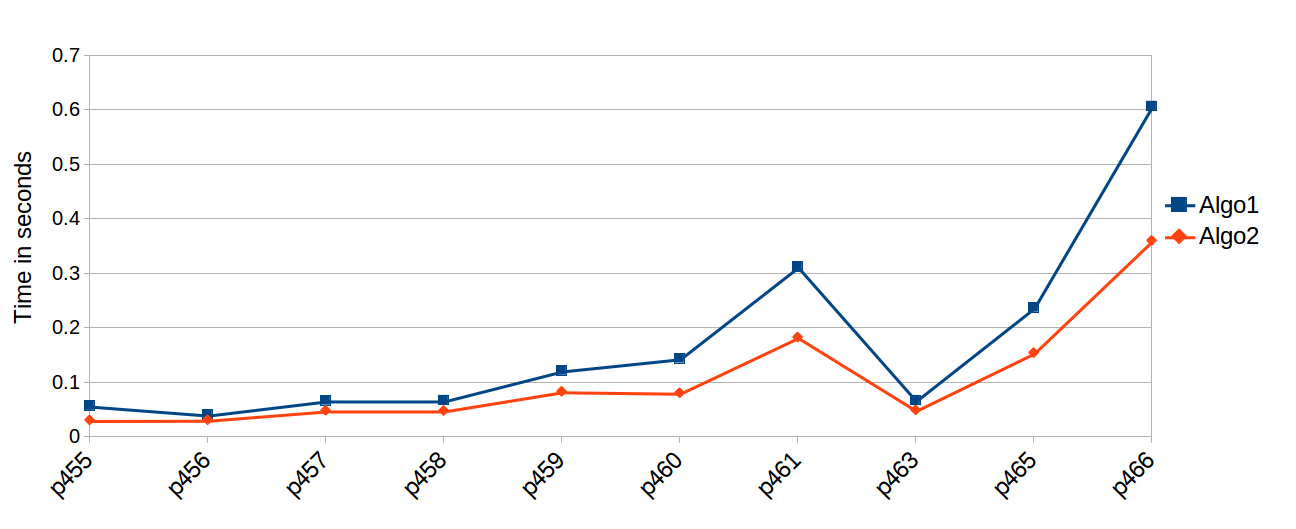
\includegraphics[scale = 0.45]{es3.png}
  \caption{Running Time comparison for Both Algorithms $algo1$ and $algo2$ on P4E dataset}
\end{figure}

\textbf{2. BCD Dataset :-} B, C, D are the instances of random generated graph with edges weights between 1 and 10. Out of these instances, we run both the algorithms on some of the instances of these dataset, as tabulated~\cite{koch}.\\ 


 \begin{figure}[H]
      \centering
    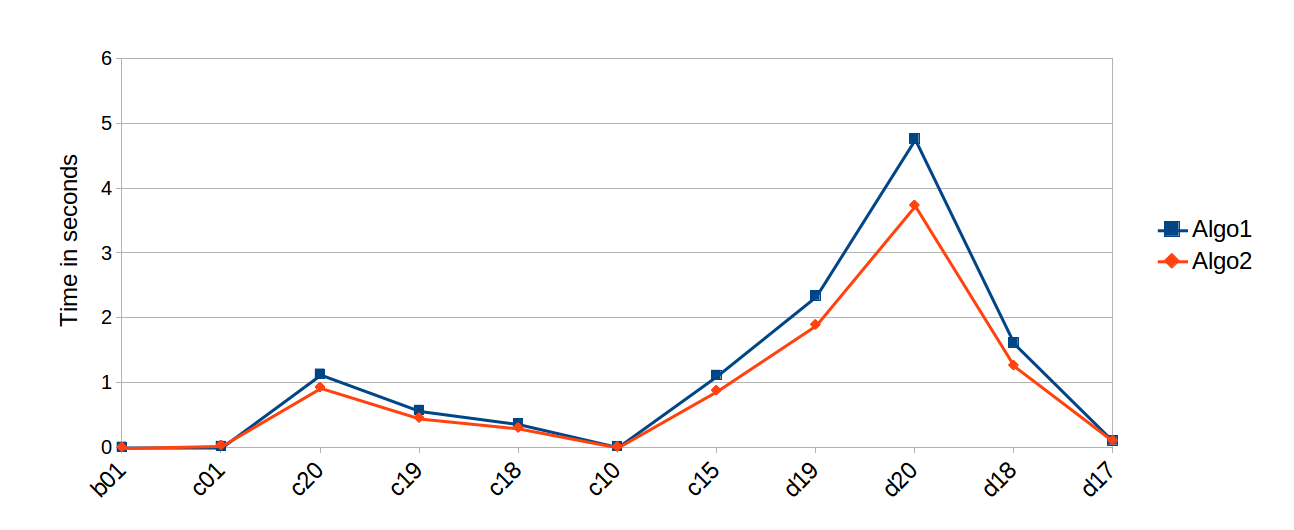
\includegraphics[scale = 0.45]{es2.png}
  \caption{Running Time Comparison for Both Algorithms $algo1$ and $algo2$ on B, C, D dataset}
\end{figure}


\begin{table}[H]
% \caption{My caption}
\label{my-label}
\begin{center}
\begin{tabular}{|l|l|l|l|l|l|}
\hline
Name & $|V|$      & $|E|$      & $|S|$      & DC         & Opt       \\ \hline
b01    &  50       &  63      &    9   &  Ls         &  82  \\ \hline
c01    &  500       &  625      &    10   &  Ps         &  144  \\ \hline
c10    &  500       &  1000      &    250   &  Ps         &  1093  \\ \hline
c15    &  500       &  2500      &    250   &  Ls         &  556  \\ \hline
c18    &  500       &  12500      &    250   &  Ps         &  113  \\ \hline
c19    &  500       &  12500      &    250   &  Ps         &  146  \\ \hline
c20    &  500       &  12500      &    250   &  Ls         &  267  \\ \hline

d17    &  1000       &  25000      &    10   &  Pm       &  23  \\ \hline
d18    &  1000       &  25000      &    167   &  Ps       &  223  \\ \hline

d19    &  1000       &  25000      &    250   &  Ps       &  310  \\ \hline
d20    &  1000       &  25000      &    500   &  Ls      &   537  \\ \hline
% P455    &  100       &  4950      &    5   &  Ps       &  1138  \\ \hline
\end{tabular}
\end{center}
\caption{B, C, D are the instances}
\end{table}

As we can see in all the cases, for all the instances B, C, D our algorithm $algo2$ taking less running time than the algorithm $algo2$.


\textbf{3. E Dataset :-} These instances are for the sparse graph that generated randomly with edges weights in between 1 to 10. DC means difficulty level of the problem.

Running times are change according to the change eigher in the number of edges or number of terminals present in the graphs. As we can see running times in figure 4.3 and figure 4.4, for the instances of table 4.1 and 4.2.  
 
\begin{table}[H]
% \caption{My caption}
\label{my-label}
\begin{center}
\begin{tabular}{|l|l|l|l|l|l|}
\hline
Name & $|V|$      & $|E|$      & $|S|$      & DC         & Opt       \\ \hline

 e01.stp &  2500      &  3125      &   5    & Ps   & 111    \\ \hline
 e02.stp &  2500      &  3125      &  10    & Ps   & 214     \\ \hline
 e03.stp &  2500      &  3125      &  417   & Ps   & 4013    \\ \hline
 e04.stp &  2500      &  3125      &  625   & PS   & 5101    \\ \hline
 e05.stp &  2500      &  3125      &  1250  & Ps   & 8128     \\ \hline
 e06.stp &  2500      &  5000      &  5     & Ps   & 73     \\ \hline
 e07.stp &  2500      &  5000      &  10    & Pm   & 145      \\ \hline
 e08.stp &  2500      &  5000      &  417   & Pm   & 2640       \\ \hline
 e09.stp &  2500      &  5000      &  625   & Pm   & 3604            \\ \hline
 e10.stp &  2500      &  5000      &  1250  & Pm   & 5600      \\ \hline
 e11.stp &  2500      &  12500     &  5     & Pm   & 34         \\ \hline
 e12.stp &  2500      &  12500     &  10    & Pm   & 67        \\ \hline
 e13.stp &  2500      &  12500     &  417   & Pm   & 1280          \\ \hline
 e14.stp &  2500      &  12500     &  625   & Pm   & 1732            \\ \hline
 e15.stp &  2500      &  12500     &  1250  & Ps   & 2784        \\ \hline
 e16.stp &  2500      &  62500     &  5     & Ph   & 15       \\ \hline
 e17.stp &  2500      &  62500     &  10    & Ph   & 25       \\ \hline
 e18.stp &  2500      &  62500     &  417   & NPh  & 564       \\ \hline
 e19.stp &  2500      &  62500     &  625   & Pm   & 758    \\ \hline
 e20.stp &  2500      &  62500     &  1250  & Ls   & 1342     \\ \hline
 
% P455    &  100       &  4950      &    5   &  Ps       &  1138  \\ \hline
\end{tabular}
\end{center}
\caption{E instances}
\end{table}


 \begin{figure}[H]
      \centering
    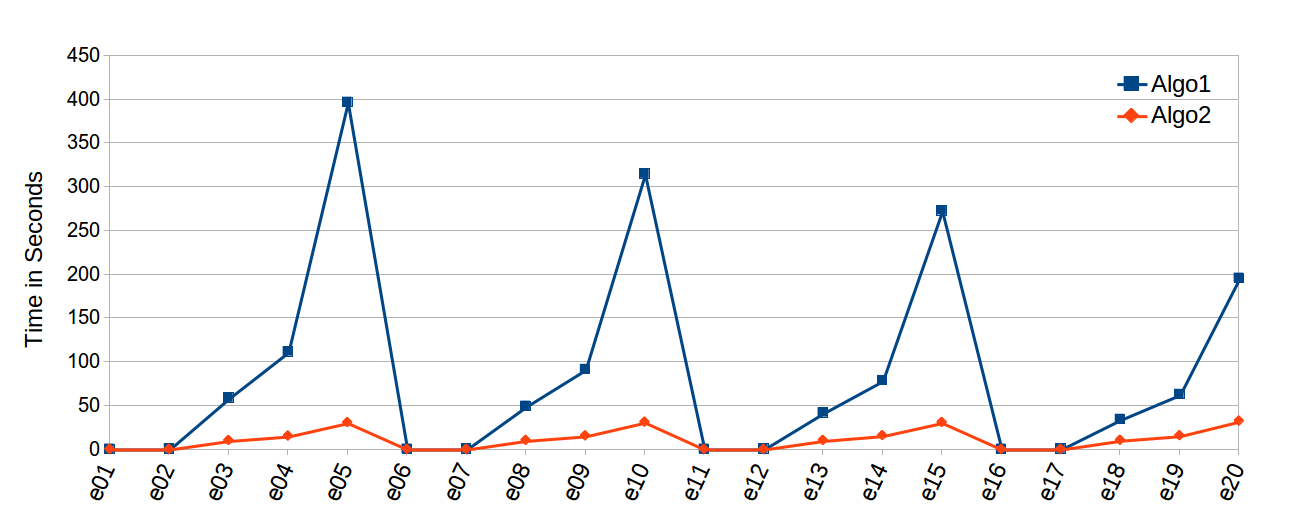
\includegraphics[scale = 0.45]{anilfinal.png}
  \caption{Running Time Comparison for Both Algorithms $algo1$ and $algo2$ on E dataset}
\end{figure}


\section{Computational Results}
Computational experiments were performed on test data set with quite different characteristics. All instance are available from the repository steinlib ~\cite{koch}. We run both the algorithms $algo1$ and $algo2$ on these instance. The running times for both the algorithms are present in the table 4.1, and table 4.2. First heuristic algorithm $algo1$ given by L. Kou, G. Markowsky, and L. Berman ~\cite{markowsky}. Second algorithm $algo2$ propose in this thesis. Both algorithms were run on the same dataset, and we calculate their running time, how much time both algorithm are taking, in almost all cases our propose algorithm is taking less time as compare to the previous heuristic algorithm. Representations in tables are as follows, $|V|$ number of vertices present in the graph, $|E|$ number of edges present in the graph, $|S|$ number of terminals present in the graph. Running time is in seconds present for both the algorithms. 

All the results in tables 4.3, 4.4, 4.5 obtained for both the programs by running these programs using G++ compiler on a machine with configuration as Intel(R) core(TM) i5-2320 CPU @ 3.00Hz 3.00 GHz processor, with RAM 4.00GM and system type 32-bit operating system. This time may change according to the machine configurations.
    

\begin{table}[H]
% \caption{My caption}
\label{my-label}
\begin{center}
\begin{tabular}{|l|l|l|l|l|l|l|l|l|}
\hline
Instance & \multicolumn{4}{l|}{Heuristic Algo1} & \multicolumn{4}{l|}{Heuristic Algo2} \\ \hline
         & $|V|$      & $|E|$      & $|S|$      & Time in Sec     & $|V|$      & $|E|$      & $|S|$     & Time in Sec    \\ \hline
     b01.stp    &  50       &    63      &     9   &  0.00369       &  50       &    63      &     9    & 0.000967        \\ \hline
     c01.stp    &  500      &    625     &     5   &  0.016047      &  500      &    625     &     5    &  0.034286    \\ \hline
     c20.stp    &  500      &   12500    &     250   &  1.13426     &  500      &   12500    &     250  &  0.928982 \\ \hline

     c19.stp    &  500      &   12500    &     150   &  0.573434      &  500       &   12500    &     150   &  0.456435 \\ \hline
     c18.stp    &  500      &   12500    &     83    &  0.369872       &  500      &   12500    &     83    &  0.30325 \\ \hline

     c16.stp    &  500      &   12500    &     5   &  0.015228      &  500      &   12500    &     5    &  0.010057 \\ \hline

     c15.stp    &  500      &   12500    &     250   &  1.11433      &  500      &   12500    &     250   &  0.879228 \\ \hline
    
     % es10fst.stp     &  18   v   &   20     &     10    &  0.021338      &  18       &   20     &     10    &  0.0582559   \\ \hline
     % att48fst.stp    &  139      &   202    &     48    &  0.123454      &  139      &   202    &     48    &  0.156677  \\ \hline
     % pr136fst.stp    &  196      &   250    &     136   &  0.408418      &  196      &   250    &     136   &  0.452413 \\ \hline
     d19.stp    &  1000      &   25000    &     250   &  2.34159      &  1000      &   25000    &     250   &  1.8951 \\ \hline
     d20.stp    &  1000      &   25000    &     500   &  4.76639      &  1000      &   25000    &     500   &  3.74008 \\ \hline
     d18.stp    &  1000      &   25000    &     167   &  1.61377      &  1000      &   25000     &     167   &  1.26696 \\ \hline
     d17.stp    &  1000      &   25000    &     10    &  0.10314       &  1000      &   25000    &      10   &  0.105337 \\ \hline
     
     % rd400fst.stp &  1001       &   1419       &   400    &  1.43076      &  1001       &   1419       &   400    &  1.50568 \\ \hline
     u574fst.stp &  990       &   1258       &   574    &  5.17052      &  990       &   1258       &   574    &  2.18517 \\ \hline
     p455.stp &  100       &   4950       &   5    &    0.0573699      &  100       &   4950       &   5    &    0.0309451 \\ \hline
     p456.stp &  100       &   4950       &   5    &    0.040837      &  100       &   4950       &   5    &    0.031431 \\ \hline
     p457.stp &  100       &   4950       &   10    &    0.0669429      &  100       &   4950       &   10    &    0.0486231 \\ \hline
     p458.stp &  100       &   4950       &   10    &    0.067569      &  100       &   4950       &   10    &    0.0483148 \\ \hline
     p459.stp &  100       &   4950       &   10    &    0.121697      &  100       &   4950       &   10    &    0.0835261 \\ \hline

     p460.stp &  100       &   4950       &   20    &    0.144033      &  100       &   4950       &   20    &    0.0809169 \\ \hline
     p461.stp &  100       &   4950       &   50   &    0.31225      &  100       &   4950       &   50    &    0.18301 \\ \hline
     p465.stp &  100       &   4950       &   40    &    0.237409      &  100       &   4950       &   40    &    0.154525 \\ \hline

     p466.stp &  200       &   19900       &   100    &    0.606883      &  200       &   19900       &   100    &    0.360251 \\ \hline

     

         % &        &        &        &           &        &        &       &          \\ \hline
         % &        &        &        &           &        &        &       &          \\ \hline
\end{tabular}
\end{center}
\caption{Detail results of computation on test instance}
\end{table}




\begin{table}[ht]
% \caption{My caption}
\label{my-label}
\begin{center}
\begin{tabular}{|l|l|l|l|l|l|l|l|l|}
\hline
Instance & \multicolumn{4}{l|}{Heuristic Algo1} & \multicolumn{4}{l|}{Heuristic Algo2} \\ \hline
         & $|V|$      & $|E|$      & $|S|$      & Time in Sec     & $|V|$      & $|E|$      & $|S|$     & Time in Sec    \\ \hline
     % d17.stp    &  1000      &   25000    &     10    &  0.10314       &  1000      &   25000    &      10   &  0.105337 \\ \hline
     es10fst15.stp &  16       &   18       &     10    &  0.71318       &  16        &   18       &      10   &  0.04878 \\ \hline
     es10fst14.stp &  24       &   32       &     10    &  0.721951       &  24        &   32       &      10   &  0.04708 \\ \hline
     es10fst13.stp &  18       &   21       &     10    &  0.72192        &  18        &   21       &      10   &  0.046977 \\ \hline

     % berlin52fst.stp & 89      &   104      &     52    &  0.318259        &  89        &   104      &    52   &  0.185827 \\ \hline
     es10fst13.stp &  18       &   21       &     10    &  0.72192        &  18        &   21       &      10   &  0.046977 \\ \hline
     es10fst13.stp &  18       &   21       &     10    &  0.72192        &  18        &   21       &      10   &  0.046977 \\ \hline
     es10fst13.stp &  18       &   21       &     10    &  0.72192        &  18        &   21       &      10   &  0.046977 \\ \hline
     es10fst13.stp &  18       &   21       &     10    &  0.72192        &  18        &   21       &      10   &  0.046977 \\ \hline
    
     % p466.stp &  200       &   19900       &   100    &    0.606883      &  200       &   19900       &   100    &    0.360251 \\ \hline

     es20fst101.stp  & 29  &   28       &   20    &  0.123531     &  29       &   28       &   20    &    0.08129 \\ \hline
     es20fst102.stp  & 29  &   28       &   20    &  0.125359     &  29       &   28       &   20    &    0.0812831 \\ \hline
     es20fst103.stp  & 27  &   26       &   20    &  0.132646     &  27       &   26       &   20    &    0.078793 \\ \hline
     es20fst104.stp  & 57  &   83       &   20    &  0.134467     &  57       &   83       &   20    &    0.0795579 \\ \hline
     es20fst105.stp  & 54  &   77       &   20    &  0.132566     &  54       &   77       &   20    &    0.0807161 \\ \hline
     es20fst106.stp  & 29  &   28       &   20    &  0.133814     &  29       &   28       &   20    &    0.0790079 \\ \hline
     es20fst111.stp  & 33  &   36       &   20    &  0.134738     &  33       &   36       &   20    &    0.0798302 \\ \hline
     es20fst113.stp  & 35  &   40       &   20    &  0.133753     &  35       &   40       &   20    &    0.0802221 \\ \hline
     es250fst01.stp  & 623  &   876       &  250    & 11.5419     & 623       &   876      &  250    &    0.893757 \\ \hline
     es250fst02.stp  & 542  &   719       &  250    & 11.5419     & 542       &   719      &  250    &    0.885769 \\ \hline

     es250fst03.stp  & 543  &   727       &  250    & 13.9157     & 543       &   727      &  250    &    0.890725 \\ \hline
     es250fst04.stp  & 604  &   842       &  250    & 11.2278     & 604       &   842      &  250    &    0.893235 \\ \hline
     es250fst05.stp  & 596  &   832       &  250    & 11.5419     & 596       &   832      &  250    &    0.891753 \\ \hline
     es250fst10.stp  & 662  &   951       &  250    & 10.8352     & 662       &   951      &  250    &    0.895662 \\ \hline
     es250fst11.stp  & 661  &   952       &  250    & 13.2844     & 661       &   952      &  250    &    0.900668 \\ \hline
     es250fst15.stp  & 713  &   1053       &  250    & 11.6048     &713       &   1053      &  250    &   0.90136 \\ \hline


         % &        &        &        &           &        &        &       &          \\ \hline
         % &        &        &        &           &        &        &       &          \\ \hline
\end{tabular}
\end{center}
\caption{Detail results of computation on test instance ES 10,20,250 fst}
\end{table}


\begin{table}[ht]
% \caption{My caption}
\label{my-label}
\begin{center}
\begin{tabular}{|l|l|l|l|l|l|l|l|l|}
\hline
Instance & \multicolumn{4}{l|}{Heuristic Algo1} & \multicolumn{4}{l|}{Heuristic Algo2} \\ \hline
         & $|V|$      & $|E|$      & $|S|$      & Time in Sec     & $|V|$      & $|E|$      & $|S|$     & Time in Sec     \\ \hline
 e01.stp &  2500      &  3125      &   5        &  0.361644       &  2500      &  3125      &   5       &  0.206146       \\ \hline
 e02.stp &  2500      &  3125      &  10        &  0.643139       &  2500      &  3125      &  10       &  0.327235       \\ \hline
 e03.stp &  2500      &  3125      &  417       &  58.8115        &  2500      &  3125      &  417      &  10.3275        \\ \hline
 e04.stp &  2500      &  3125      &  625       &  111.695        &  2500      &  3125      &  625      &  15.4805        \\ \hline
 e05.stp &  2500      &  3125      &  1250      &  396.873        &  2500      &  3125      &  1250     &  30.8221        \\ \hline
 e06.stp &  2500      &  5000      &  5         &  0.356108       &  2500      &  3125      &  5        &  0.205941       \\ \hline
 e07.stp &  2500      &  5000      &  10        &  0.628921       &  2500      &  5000      &  10       &  0.330493       \\ \hline
 e08.stp &  2500      &  5000      &  417       &  49.4262        &  2500      &  5000      &  417      &  10.4627        \\ \hline
 e09.stp &  2500      &  5000      &  625       &  91.5182        &  2500      &  5000      &  625      &  15.6537        \\ \hline
 e10.stp &  2500      &  5000      &  1250      &  314.90         &  2500      &  5000b     &  1250     &  31.3128        \\ \hline
 e11.stp &  2500      &  12500     &  5         &  0.349082       &  2500      &  12500     &  5        &  0.202747       \\ \hline
 e12.stp &  2500      &  12500     &  10        &  0.607044       &  2500      &  12500     &  10       &  0.32562        \\ \hline
 e13.stp &  2500      &  12500     &  417       &  41.892         &  2500      &  12500     &  417      &  10.4017        \\ \hline
 e14.stp &  2500      &  12500     &  625       &  78.7861        &  2500      &  12500     &  625      &  15.9379        \\ \hline
 e15.stp &  2500      &  12500     &  1250      &  272.956        &  2500      &  12500     &  1250     &  30.9364        \\ \hline
 e16.stp &  2500      &  62500     &  5         &  0.337468       &  2500      &  62500     &  5        &  0.205354       \\ \hline
 e17.stp &  2500      &  62500     &  10        &  0.595741       &  2500      &  62500     &  10       &  0.331765       \\ \hline
 e18.stp &  2500      &  62500     &  417       &  34.4145        &  2500      &  62500     &  417      &  10.6498        \\ \hline
 e19.stp &  2500      &  62500     &  625       &  62.9514        &  2500      &  62500     &  625      &  15.8446        \\ \hline
 e20.stp &  2500      &  62500     &  1250      &  195.743        &  2500      &  62500     &  1250     &  32.5236        \\ \hline
 
\end{tabular}
\end{center}
\caption{Detail results of computation on test instance E}
\end{table}

% \section{Conclusion} All the results in tables 4.3, 4.4, 4.5 obtained for both the programs by running these programs using G++ compiler on a machine with configuration as Intel(R) core(TM) i5-2320 CPU @ 3.00Hz 3.00 GHz processor, with RAM 4.00GM and system type 32-bit operating system. This time may change according to the machine configurations.



%\chapter{Tree Spanners} \label{ch_exact}
%Chapter 4
%%%%%%%%%%%%%%%%%%%%%%%%%%%%%%%%%%%%%%%%%%%%%%%%%%%%%%%%%%%%%%%%%%%%%%%%%%%%%%%%%%%%%%%%%%%%%%%%%%%%%%%%%%%%%%%%%%%%%%


\chapter{CONCLUSION AND FUTURE WORK} \label{ch_concl}
%Chapter 6
%%%%%%%%%%%%%%%%%%%%%%%%%%%%%%%%%%%%%%%%%%%%%%%%%%%%%%%%%%%%%%%%%%%%%%%%%%%%%%%%%%%%%%%%%%%%%%%%%%%%%%%%%%%%%%%%%%%%%%%%%
\section{Conclusion and Future Work}
 In this work, we have designed a heuristic approximation algorithm for Steiner tree by using all-pairs shortest-path algorithm, with the help of this algorithm, we have came to a some better algorithm whose running time is better then previous heuristic algorithm presented by L.~Kou, G. Markowsky, and L, $A$ $Fast$ $Algorithm$ $for$ $Steiner$ $Tree$ ~\cite{markowsky}, running time of this algorithm was $O(|S||V|^2)$. where $|S|$ is the number of terminals and $|V|$ is the number of vertices in the graph $G$. In this algorithm running time mainly taken by the first step, rest of the step are taking a running time of some what smaller then that, so our thinking were how to reduce the running time for this step 1 only, and get a some better running time complexity. For that think we used all-pairs shortest-path problem, and we come up with a better running time complexity i.e., $O(|S||V|log|V|)$ for the graph the graph which have order of edges $O(E)$ $\leq$ $|V|log|V|$ and $O(|S||V|log|V| + |E||S|)$ for the other graph this running time is depend on the order of edges present in the graphs. Computational results presented by our heuristic algorithm is competitive with the previous heuristic algorithm for the Steiner tree. For some instances our algorithm fail to get better running time, where the order of edges is more than the $|V|log|V|$. In the implementation of algorithms, we used C++ as language for implementation. One can participate in the DIMACS implementation challenge with good implementations.
  
 % \section{Future Work} 

 %%%%%%%%%%%%%%%%%%%%%%%%%%%%%%%%%%%%%%%%%%%%%%%%%%%%%%%%%%%%%%%%%%%%%%%%%%%%%%%%%%%%%%%%%%%%%%%%%%%%%%%%%%%%%%%%%%%%%%%


%%%%%%%%%%%%%%%%%%%%%%%%%%%%%%%%%%%%%%%%%%%%%%%%%%%%%%%%%%%%%%%%%%%%%%%
% List of papers
% % % % % %  % % % % 
%
%
%
%
%
% 
%%%%%%%%%%%%%%%%%%%%%%%%%%%%%%%%%%%%%%%%%%%%%%%%%%%%%%%%%%%%%%%%%%%%%%%%%
% Bibliography.
\pagebreak
\nocite{*}
\begin{singlespace}
  \begin{small}
	\bibliographystyle{plain}
	\bibliography{thesis}
%	\bibliography{iccad}
  \end{small}
\end{singlespace}

%%%%%%%%%%%%%%%%%%%%%%%%%%%%%%%%%%%%%%%%%%%%%%%%%%%%%%%%%%%%%%%%%%%%%%%%%%%%%


\end{document}
